\chapter{Evidence for UID effects on omissions in fragments}
\label{sec:chapter-infotheory-experiments}

This chapter presents two experiments which investigate the predictions of the UID-based account of fragment usage.%
%
\footnote{Experiment \ref{exp:scripts-rating} has been published in \citet{lemke.etal2021} and experiment \ref{exp:scripts-production} has been published in \citet{lemke.etal2020} and \citet{lemke.etal2021a}.}\afterfn%
%
This account makes the three testable predictions in \Next. \Next[a] and \Next[b] are specific to UID\is{Uniform Information Density}, whereas \Next[c] can be analyzed either as an implication of \Next[a] and \Next[b] or as the result of efficient source coding\is{Source coding}.

\ex. Predictions of UID\is{Uniform Information Density} on fragments
\a. \textit{Avoid troughs}: The more likely a word is in context, the more likely it is to be omitted (within the limits of grammar).\label{ex:uid-pred-troughs}
 \b.\textit{Avoid peaks}: Uninformative\is{Shannon information} words can be inserted before very informative\is{Shannon information} words in order to lower the surprisal\is{Shannon information} of the latter (within the limits of grammar). \label{ex:uid-pred-peaks}
 \c. \textit{Densification}: Shorter encodings, like fragments, are preferred in predictive contexts.\label{ex:uid-pred-density}

The experiments investigate these issues at the case of discourse-initial fragments\is{Fragment, discourse-initial}, which are the most uncontroversial instances of fragments. Since these fragments lack linguistic antecedents, the predictability of words within them mostly constrained by extralinguistic context\is{Context, extralinguistic}. In order to quantify effects of extralinguistic context\is{Context, extralinguistic} on the predictability of utterances and words within them,  both experiments rely on script knowledge\is{Script knowledge} \citep{schank.abelson1977} as an approximation to extralinguistic context\is{Context, extralinguistic}. Scripts\is{Script knowledge} trigger expectations about upcoming events\is{Event chain} and can be used to modulate the predictability of utterances that are related to these events\is{Context, extralinguistic}. Furthermore, there is a crowdsourced corpus\is{Corpus} of script knowledge\is{Script knowledge} available that can be used to precisely quantify this predictability. 

\is{Context, extralinguistic|(}Both experiments manipulate the likelihood of utterances with context stories like \Next, which are based on event probabilities\is{Event chain} extracted from the DeScript corpus\is{Corpus} of script knowledge\is{Script knowledge} \citep{wanzare.etal2016}. For instance, in context of this story, the most likely event to follow is that of pouring the pasta into the boiling water, hence I assume that utterances that refer to this event, like \Next[a] are more likely than those referring to events which are unpredictable in the script\is{Script knowledge} corpus\is{Corpus}.\is{Context, extralinguistic|)}

\ex. Annika and Jenny want to cook pasta. Annika put a pot with water on the stove. Then she turned the stove on. After a few minutes, the water started to boil.
\a. Pour the pasta into the pot. \hfill Predictable
\b. Set the table. \hfill Unpredictable

Experiment \ref{exp:scripts-rating} compares the acceptability\is{Acceptability rating task} of the sentences in \Last[a,b] to that of DP\is{Determiner phrase} fragments derived from these sentences. Given clause \LLast[c], UID\is{Uniform Information Density} predicts a relatively stronger preference for fragments in case of the predictable utterance \Last[a]  than in case of \Last[b]. Experiment \ref{exp:scripts-production} uses the same context stories to elicit a data set with a production task\is{Production task} that is suitable for investigating the more fine-grained predictions in \LLast[a] and \LLast[b]. The presence of ellipses in the data collected in experiment \ref{exp:scripts-production} requires a new method to estimate surprisal\is{Shannon information}. My method extends the surprisal\is{Shannon information} estimation technique proposed by \citet{hale2001} to elliptical data by allowing for an arbitrary number of omissions between words.

This chapter is organized as follows. In Section \ref{sec:infotheory-scripts} I propose scripts\is{Script knowledge} as an approximation to extralinguistic context\is{Context, extralinguistic} and describe how I created experimental materials based on the DeScript corpus\is{Corpus} \citep{wanzare.etal2016}. Sections \ref{sec:scripts-rating} and \ref{sec:scripts-production} present the experiments, and Section \ref{sec:scripts-discussion} summarizes the main results.

\section{Scripts as a model of extralinguistic context}
\label{sec:infotheory-scripts}

In information-theoretic\is{Information theory} research on language, the surprisal\is{Shannon information} of words is most frequently estimated from corpora\is{Corpus} using statistical language models.%
%
\footnote{Other methods include approximating the surprisal\is{Shannon information} of function words with the likelihood of particular constructions, such as relative clauses \citep{levy.jaeger2007} or complement clauses\is{Complement clause} \citep{jaeger2010}. This can be done either by calculating e.g. the subcategorization preferences of verbs from previously parsed corpora\is{Corpus} \citep{jaeger2010} or by using probabilistic parsers, which operate on part of speech annotations and calculate the likelihood of the syntactic construction investigated \citep{levy.jaeger2007}. Furthermore, other authors have simply stipulated that, everything else being equal, expressions that occur later in a sentence or text are more predictable, because previous material narrows the range of possible continuations. See e.g. \citet{fenk-oczlon1989}, \citet{fenk-oczlon1990} and \citet{genzel.charniak2002} for studies that (partially) relied on this assumption and \citet[1147]{levy2008} for empirical evidence.
}\afterfn%
%
Previous studies in the field relied mostly on \textit{n}-gram models\is{N-gram language model}, which model the context of a word $w_{i}$ as the $n-1$ words that precede it. Unigram models\is{Unigram language model} consider only the overall frequency of $w_{i}$, bigram models\is{Bigram language model} return the conditional probability $p(w_i \mathbin{|} w_{i-1})$, trigram models\is{Trigram language model} use  $p(w_i \mathbin{|} w_{i-2}\; w_{i-1})$, and so on. By restricting context to a few words at most, \textit{n}-gram models\is{N-gram language model} are only very coarse approximations to the models of context that human interlocutors probably construct. Even though there are currently more sophisticated language modeling techniques,%
%
\footnote{Some models take into account hierarchical structure \citep{stolcke1995, hale2001,roark2001, levy2008} or even material contained in previous sentences \citep{iyer.ostendorf1996, oualil.etal2016, oualil.etal2017, singh.etal2016a, grave.etal2017, khandelwal.etal2018, devlin.etal2019}.}\afterfn%
%
they are also not suitable to estimate surprisal in discourse-initial\is{Fragment, discourse initial} fragments: Since there is no or only little context in these utterances, the likelihood of words within them is determined by extralinguistic context\is{Context, extralinguistic} to a large extent. Text corpora\is{Corpus} do not contain information\is{Shannon information} about extralinguistic context\is{Context, extralinguistic}, so the models cannot quantify its effect on the likelihood of words. Therefore, investigating predictability effects on fragments place requires a model of extralinguistic context\is{Context, extralinguistic}. As I anticipated in the preceding section, I use script knowledge\is{Script knowledge} for this purpose.

Scripts\is{Script knowledge} \citep{schank.abelson1977} are stereotypical representations of everyday situations, which contain information\is{Shannon information} about the default ordering of events as well as participants and objects involved \citep{bower.etal1979}. Three properties of fragments make scripts\is{Script knowledge} particularly suitable as an approximation%
%
\footnote{It shall be noted that scripts\is{Script knowledge} are an approximation to extralinguistic context\is{Context, extralinguistic} rather than a complete models thereof. Context is not only determined by script knowledge\is{Script knowledge}, since non-conventionalized, visual or other sensory information\is{Shannon information} will also have an effect on expectations about upcoming events and utterances. In the taxi scenario, the pedestrian might be wheeling a bike, therefore it becomes relatively unlikely that he would ask for a taxi ride. However, the effect of such properties of context is difficult to quantify and in my stimuli I avoid the mention of such unexpected referents.}\afterfn%
%
to extralinguistic context\is{Context, extralinguistic}: First, scripts\is{Script knowledge} are accessed during text comprehension in order to retrieve implicit material, second, at least some scripts\is{Script knowledge} are shared by most speakers of a language, and third, people predict upcoming events based on script knowledge\is{Script knowledge}. In experimental settings, it can be assumed that scripts\is{Script knowledge} which are shared by a majority of the population trigger similar expectations for most of the participants. This allows for controlling and manipulating context-driven expectations: In the taxi scenario an utterance like \textit{take me to \dots} will be likely. Furthermore, there are script corpora\is{Corpus} available which consist in descriptions of the stereotypical time-course of scripts\is{Script knowledge} provided by a large number of participants. Based on these corpora\is{Corpus}, it is possible to build probabilistic models of context\is{Event chain} which can be used to precisely estimate event probabilities\is{Event chain}. 

This section describes the model of extralinguistic context\is{Context, extralinguistic} based on the DeScript script knowledge\is{Script knowledge} corpus\is{Corpus} \citep{wanzare.etal2016} that underlies the stimuli for experiments \ref{exp:scripts-rating} and \ref{exp:scripts-production}. Section \ref{sec:infotheory-scripts-scrkn} introduces the concept of script as defined by \citet{schank.abelson1977} and briefly discusses previous psychological evidence that scripts\is{Script knowledge} indeed prime upcoming events. Section \ref{sec:infotheory-script-event-chains} presents the approach I used for estimating event probabilities\is{Event chain} from the DeScript corpus\is{Corpus} of script knowledge\is{Script knowledge} \citep{wanzare.etal2016}.

\subsection{Script knowledge} \label{sec:infotheory-scripts-scrkn}
\is{Script knowledge|(}The concept of \textit{script} has been established by \citet{schank.abelson1977} as an extension of the idea of \textit{frames} developed by \citet{minsky1974}. In principle, a script\is{Script knowledge} can be defined as the mental representation of a stereotypical everyday activity, such as grocery shopping, visiting a doctor, eating in a restaurant or attending a lecture \citep{bower.etal1979}. \citet{schank.abelson1977} attribute scripts\is{Script knowledge} a central role in text comprehension, which consists in filling the gap between what is explicitly said and what is understood. They exemplify this at the case of a short story about visiting a restaurant \Next. 

\ex. John went to a restaurant. He asked the waitress for coq au vin. He paid the check and left. \hfill \citep[38]{schank.abelson1977} \label{ex:scripts-restaurant-ex}

Although the story omits many details, for instance that John sat down at a table, read the menu, ordered something to drink, and even the central act of eating the dish that he ordered, a hearer will infer these events from knowledge about the stereotypical time-course of eating at a restaurant as well as about the people and objects involved. Events that are highly predictable at some point in the script\is{Script knowledge} can remain implicit and will nevertheless be integrated in the hearer's representation of the described situation.

\subsubsection{The structure of scripts}
In order to quantify the likelihood of an event at a specific point in the script\is{Script knowledge} it is crucial to know how its internal structure looks like. This concerns the hierarchical structure of the script\is{Script knowledge} as well as the ordering of events: If scripts\is{Script knowledge} were fully ordered sequences of events\is{Event chain}, each event would deterministically indicate what happens next. In what follows, I briefly sketch the structure of scripts\is{Script knowledge} as described in \citet{schank.abelson1977}, which differs in some aspects from the representations of scripts\is{Script knowledge} on which my stimuli are based. Figure \ref{fig:restaurant-script-schank.abelson} shows the structure of (a part of) the restaurant script\is{Script knowledge} according to \citet{schank.abelson1977}.%
% 
\footnote{Note that I replaced the original conceptual dependency theory \citep{schank1975} representations of scripts\is{Script knowledge} by their natural language counterparts for expository purposes.}\afterfn%
%

\begin{figure}
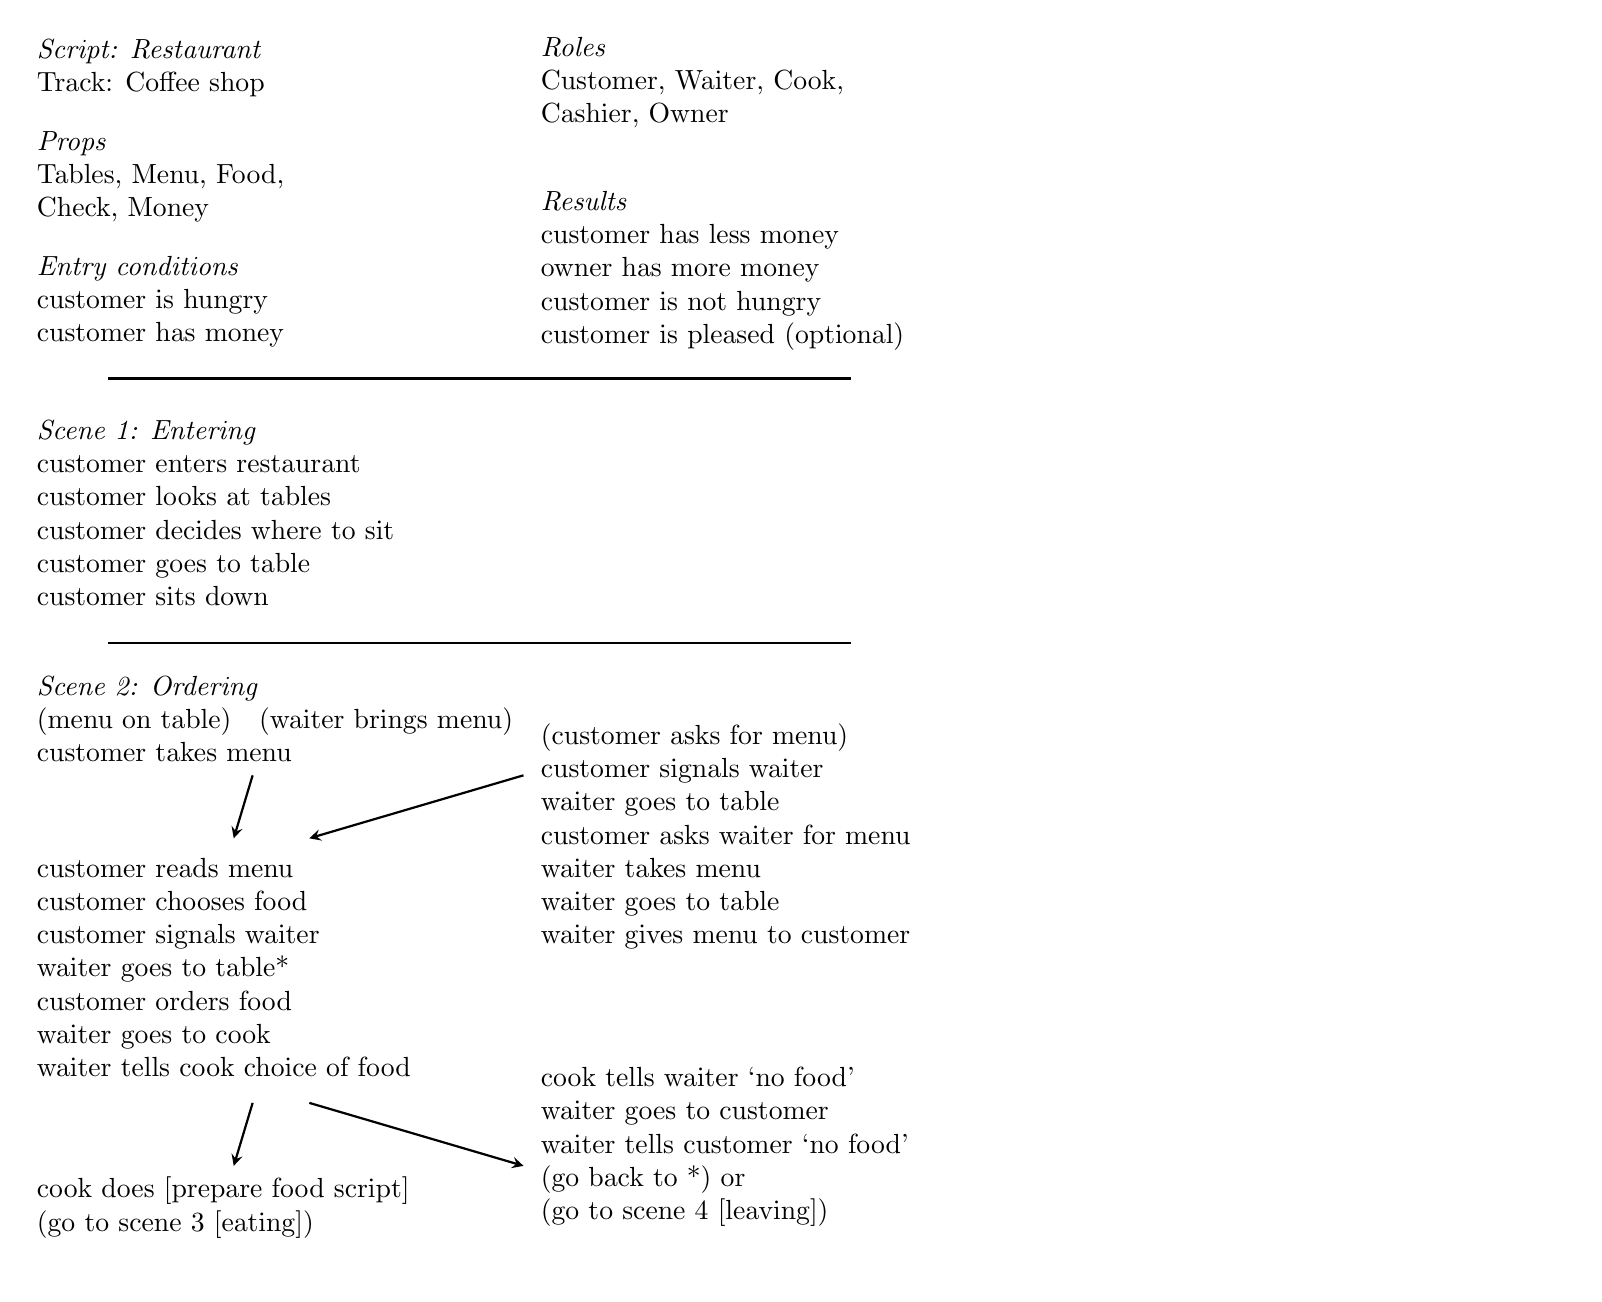
\begin{tikzpicture}[scale=.8]

\node (header) at (0,7.7) {
\begin{minipage}{13cm}
\textit{Script: Restaurant}\\
Track: Coffee shop\\
\end{minipage}
};

\node (props) at (0,6.2) {
\begin{minipage}{13cm}
\textit{Props}\\
Tables, Menu, Food, \\
Check, Money
\end{minipage}
};

\node (roles) at (8,7.7) {
\begin{minipage}{13cm}
\textit{Roles}\\
Customer, Waiter, Cook, \\
Cashier, Owner
\end{minipage}
};

\node (conditions) at (0,4) {
\begin{minipage}{13cm}
\textit{Entry conditions}\\
customer is hungry\\
customer has money\\
\end{minipage}
};

\node (results) at (8,4.5) {
\begin{minipage}{13cm}
\textit{Results}\\
customer has less money\\
owner has more money\\
customer is not hungry\\
customer is pleased (optional)\\
\end{minipage}
};

\node (entering) at (0,0.6) {
\begin{minipage}{13cm}
\textit{Scene 1: Entering}\\
customer enters restaurant\\
customer looks at tables\\
customer decides where to sit\\
customer goes to table\\
customer sits down\\
\end{minipage}
};

\node (ordering1) at (0,-2.4) {
\begin{minipage}{13cm}
\textit{Scene 2: Ordering}\\
(menu on table)~~~(waiter brings menu)\\
customer takes menu
\end{minipage}
};

\node (ordering2) at (8,-4.49) {
\begin{minipage}{13cm}
(customer asks for menu)\\
customer signals waiter\\
waiter goes to table\\
customer asks waiter for menu\\
waiter takes menu\\
waiter goes to table\\
waiter gives menu to customer\\
\end{minipage}
};

\node (ordering3) at (0,-6.5) {
\begin{minipage}{13cm}
~~\\
customer reads menu\\
customer chooses food\\
customer signals waiter\\
waiter goes to table*\\
customer orders food\\
waiter goes to cook\\
waiter tells cook choice of food  \\
\end{minipage}
};

\node (ordering4) at (8,-9.2) {
\begin{minipage}{13cm}
cook tells waiter `no food'\\
waiter goes to customer\\
waiter tells customer `no food'\\
(go back to *) or\\
(go to scene 4 [leaving])
\end{minipage}
};

\node (ordering5) at (0,-10.37) {
\begin{minipage}{13cm}
cook does [prepare food script]\\
(go to scene 3 [eating])\\
\end{minipage}
};

\draw[thick] (-7,3) -- (4.8,3);
\draw[thick] (-7,-1.2) -- (4.8,-1.2);
\draw[thick, -stealth] (-4.7,-3.3) -- (-5,-4.3);
\draw[thick, -stealth] (-.4,-3.3) -- (-3.8,-4.3);
\draw[thick, -stealth] (-4.7,-8.5) -- (-5,-9.5);
\draw[thick, -stealth] (-3.8,-8.5) -- (-0.4,-9.5);

\end{tikzpicture}
\caption{Extract of the restaurant script based on \citet[43]{schank.abelson1977}. For expository purposes, I replaced the CDT representations by natural language counterparts and simplified Scene 2.\label{fig:restaurant-script-schank.abelson}}
\end{figure}

First, each script\is{Script knowledge} has a \textit{header} (``Restaurant''), a set of \textit{roles} identifying the participants involved in the script\is{Script knowledge}, and a set of \textit{props}, i.e. objects that typically appear in that script\is{Script knowledge}. A script\is{Script knowledge} can have several \textit{tracks}, for instance, \citet[40-41]{schank.abelson1977} distinguish a ``fancy restaurant track'' and a ``fast-food track'' in order to account for differing sets of props, roles, events, and ordering thereof depending on the type of restaurant. Scripts\is{Script knowledge} are activated by their necessary \textit{entry conditions} and lead to a set of \textit{results}, some of which might be optional. If the entry conditions are not satisfied, e.g. when a customer who is not hungry or who has no money goes to the restaurant, the events will not follow their stereotypical time-course, so that applying the script\is{Script knowledge} will not yield a benefit in comprehension. The results follow from the application of a script\is{Script knowledge} or a particular version thereof.

\citet{schank.abelson1977} assume that script\is{Script knowledge} events are hierarchically grouped into \textit{scenes}. For instance, they divide the restaurant script\is{Script knowledge} into entering, ordering, eating and exiting scenes.%
%
\footnote{There is some experimental evidence that scripts\is{Script knowledge} are indeed represented as hierarchical structures in memory. For instance, \citet{bower.etal1979} report a segmentation task on script\is{Script knowledge} data suggesting that subjects agree to a large extent on the placement of boundaries between script\is{Script knowledge} events. They argue that this indicates a natural segmentation of scripts\is{Script knowledge} into scenes. \citet{abbott.etal1985} present a memory recall task that evidences a distinction in asymmetric priming between script\is{Script knowledge} events and scene headers: While the former facilitate the recall of the latter, this does not hold vice versa. More recently, a similar structure has been assumed by \citet{cooper.shallice2000} in order to model errors in script\is{Script knowledge}-based behavior, but see \citet{botvinick.plaut2004} for a non-hierarchical account. As all of my materials involve a sequence of three consecutive script\is{Script knowledge} events on the same granularity level, both flat and hierarchical script\is{Script knowledge} models predict that the next event will be activated. I hence remain agnostic with respect to the precise representation of script knowledge\is{Script knowledge} in memory.}\afterfn%
%
Each scene in turn comprises a set of (partially) ordered events. Although many events in the restaurant follow each other obligatorily, the ordering of events within a scene is neither complete, nor is the path to be followed through each scene fully linear. The \textit{entering} scene is described as fully linear, but the \textit{ordering} scene can develop in different ways depending on whether the menu is on the table when the customers sit down. If the waiter does not bring food to the customer, it is either possible to return to the food choice event or to skip the \textit{eating} scene and proceed with \textit{leaving}. I address this partially nonlinear ordering of events by estimating their likelihood in the context of the previous one(s) from a script\is{Script knowledge} corpus\is{Corpus}.

\subsubsection{Scripts as primes for upcoming material}
This brief sketch of \citepos{schank.abelson1977} view on scripts\is{Script knowledge} suggests that scripts\is{Script knowledge} are a promising approximation to extralinguistic context\is{Context, extralinguistic}. Since scripts\is{Script knowledge} about everyday events are shared by a wide part of the population, and their representation is relatively homogeneous between individuals \citep{bower.etal1979}, it is reasonable to assume that a script\is{Script knowledge} evokes similar predictions within at least most of the participants in an experiment. \is{Event chain|(}As I discuss in greater detail in the next section, the basic idea underlying my experiments is to manipulate the likelihood of a target event with a script\is{Script knowledge}-based context story. \Next exemplifies the structure of a sample item used in experiment \ref{exp:scripts-rating} for the pasta cooking script\is{Script knowledge}. The context story consists of a  sentence referring to the script\is{Script knowledge} title \Next[a] and a sequence of the three immediately preceding events \Next[b-d].%
%
\footnote{For details on how this structure is generated and why other potential script\is{Script knowledge} events such as \textit{grab a large pot} or \textit{open the pasta package} are not included, see Section \ref{sec:infotheory-scr-corpus-preprocessing}.}\afterfn% 
%
\is{Event chain|)}Given this context story, I expect script\is{Script knowledge} events \Next[e] that are likely in that context to be more predictable than non-script events \Next[f]. This setting allows for the investigation of the hypothesis that utterances referring to predictable events are more likely to be reduced.

\ex.  \label{ex:scripts-item-abstract}
\a. cook pasta \hfill Script title
    \b. put pot with water on stove \hfill Context event 1
    \c. turn stove on\hfill Context event 2
    \d. water boils\hfill Context event 3
    \e. pour pasta into pot\hfill Target event
    \f. set table \hfill Non-script event

Based on \citepos{schank.abelson1977} theory, it seems natural to assume that \Last[e] is predictable in  the context of \Last[a-d], however, it needs to be empirically shown that this is indeed the case. Fortunately, a large bulk of experimental studies indicates that text comprehension involves the generation of predictive inferences about upcoming material \citep[see e.g.][]{bower.etal1979, mckoon.ratcliff1986, vandenbroek1994, vandermeer.etal2002, nuthmann.vandermeer2005,camblin.etal2007, otten.vanberkum2007, hare.etal2009, bicknell.etal2010, matsuki.etal2011,metusalem.etal2012, delogu.etal2018}. For instance, \citet{bower.etal1979} find that sentences referring to script\is{Script knowledge} events are read faster when they follow the immediately preceding event in the script\is{Script knowledge}, as compared to contexts where one or two events in between them are omitted. This suggests that subjects generate expectations that constrain processing\is{Processing effort} as they read script\is{Script knowledge}-based stories. More recently, \citet{vandermeer.etal2002} show that the priming effect of script knowledge\is{Script knowledge} is stronger for upcoming events. Taken together, previous research on script knowledge\is{Script knowledge} predicts that the context story in \Last[a-d] will indeed prime the target event in \Last[e] as compared to the unrelated \Last[f].\is{Script knowledge|)} In what follows, I explain how the likelihood of an event in context was calculated based on the DeScript corpus\is{Corpus} of script knowledge\is{Script knowledge}.

\subsection{Estimating event surprisal from script corpora}
\label{sec:infotheory-script-event-chains}

\subsubsection{Scripts as probabilistic event chains}
\is{Event chain|(}The script\is{Script knowledge} representations underlying the materials for experiments \ref{exp:scripts-rating} and \ref{exp:scripts-production} model scripts\is{Script knowledge} as probabilistic networks rather than as linear event sequences, as most of the previous work on scripts\is{Script knowledge} did. In such a network, each event is assigned a state $e_i$ which has a transition probability to another state $e_j$. The transition probability $p(e_j\mathbin{|}e_i)$ indicates the likelihood of $e_j$ to follow $e_i$ and can be estimated for each pair of states $\langle e_i,e_j\rangle$ {}in the total set of states that is determined by the script\is{Script knowledge}. The transition probabilities can range from 0, i.e. $e_j$ never follows $e_i$, to 1 in case $e_j$ always follows $e_i$. Figure \ref{fig:script-abstract} shows a part the abstract representation of the pasta scenario. Based on the transition probabilities it is possible to extract a linear sequence of the most likely events to follow each other even though the underlying structure itself is nonlinear. For instance, the four events marked in grey in Figure \ref{fig:script-abstract} were used to build the item for the pasta scenario given in \ref{ex:scripts-item-abstract}.\is{Event chain|)}

\begin{figure}[t]
  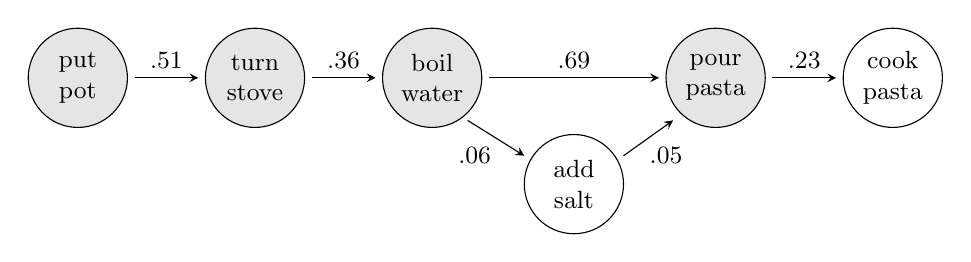
\begin{tikzpicture}[scale=.9]
{\small
\fill [black!10!] (0,0) circle [radius=.7];
\fill [black!10!] (2.5,0) circle [radius=.7];
\fill [black!10!] (5,0) circle [radius=.7];
\fill [black!10!] (9,0) circle [radius=.7];
\fill [white] (7,-1.5) circle [radius=.7];
\fill [white] (11.5,0) circle [radius=.7];

\draw [black] (0,0) circle [radius=.7] node[align=center]{put\\pot};
\draw [black] (2.5,0) circle [radius=.7] node[align=center]{turn\\stove};
\draw [black] (5,0) circle [radius=.7] node[align=center]{boil\\water};
\draw [black] (9,0) circle [radius=.7] node[align=center]{pour\\pasta};
\draw [black] (7,-1.5) circle [radius=.7] node[align=center]{add\\salt};
\draw [black] (11.5,0) circle [radius=.7] node[align=center]{cook\\pasta};

\draw [-stealth] (.8,0) -- (1.7,0) node at (1.25,.25){.51};
\draw [-stealth] (3.3,0) -- (4.2,0) node at (3.75,.25){.36};
\draw [-stealth] (5.8,0) -- (8.2,0) node at (7,.25){.69};
\draw [-stealth] (9.8,0) -- (10.7,0) node at (10.25,.25){.23};
\draw [-stealth] (5.5,-0.6) -- (6.3,-1.1) node at (5.6,-1.1){.06};
\draw [-stealth] (7.7,-1.1) -- (8.4,-0.6) node at (8.3,-1.1){.05};

}
\end{tikzpicture}
 \caption{Sample event chain with transition probabilities between events estimated from the preprocessed DeScript data. The four events marked in grey were used in the item for the pasta scenario in experiment \ref{exp:scripts-rating}.\label{fig:script-abstract}}
\end{figure}

The usage of probabilistic structures has conceptual and methodological advantages over hand-crafted script\is{Script knowledge} structures like the restaurant script\is{Script knowledge} sketched in Figure \ref{fig:restaurant-script-schank.abelson} above. First, probabilistic structures might be more empirically appropriate descriptions of  differing representations of the same script\is{Script knowledge} within the population. Intuitions of an individual researcher might deviate from the overall most likely time-course of events, and averaging over data from about 100 contributors to the corpus\is{Corpus} data for each script\is{Script knowledge} is a better approximation to the general expectations about a script\is{Script knowledge}. Second, probabilistic event chain\is{Event chain}s model the uncertainty about upcoming events in the script\is{Script knowledge}. Even in the detailed sketch of the restaurant script\is{Script knowledge} by \citet{schank.abelson1977} there is no fully linear order but several branchings, for instance the waiter might serve the customer the intended dish or not. Speakers might have probabilistic expectations about which of these continuations is more likely, and these expectations must be quantified when it comes to estimating the likelihood of upcoming events. This uncertainty is a property of scripts\is{Script knowledge} even if a single speaker has a fully deterministic view on it. For instance, a person who always prepares scrambled eggs in the same way has knowledge about how others do it. If scripts\is{Script knowledge} are used in the comprehension of new stories, it seems reasonable to rely not only on individual preferences: A hearer will expect with a certain probability that bacon, vegetables or spices are added. 
Finally, transition probabilities between events can be estimated from script\is{Script knowledge} corpora\is{Corpus}. In contrast, if the ordering between two events is reverted only once in the corpus\is{Corpus}, a linear order cannot be established. Taken together, all of these issues favor the resort to probabilistic representations of scripts\is{Script knowledge} that I use in my studies. In the remainder of Section \ref{sec:infotheory-scripts}, I describe the procedure that I used to extract context stories like that given above from the DeScript corpus\is{Corpus} of script knowledge\is{Script knowledge} \citep{wanzare.etal2016}.

\subsubsection{Selection of scripts from the DeScript corpus}
The experiments presented in this chapter are based on data extracted from the DeScript corpus\is{Corpus} \citep{wanzare.etal2016}. DeScript has been crowdsourced on Amazon Mechanical Turk and comprises about 100 event-sequence descriptions (ESD\is{Event sequence description}s) by native speakers of English\is{English} for each of 40 scripts\is{Script knowledge}. The corpus\is{Corpus} is freely available in XML format and is partially annotated for coreferences between script\is{Script knowledge} events. The scripts\is{Script knowledge} contained in the corpus\is{Corpus} differ both in their internal complexity (e.g. \textit{washing dishes} and \textit{going to a funeral}), that is, variation between (the number of) events and their order as well as with respect to the number of participants involved. 

The corpus also contains both what \citet{schank.abelson1977} termed situational and instrumental scripts\is{Script knowledge}, between which \citet{schank.abelson1977} assume a categorical distinction. Instrumental scripts\is{Script knowledge} ``usually'' have only one participant \citep[65]{schank.abelson1977}, and the order of events in the script\is{Script knowledge} is more fixed than in situational ones. As examples of instrumental scripts\is{Script knowledge}, they list scripts\is{Script knowledge} like \textit{lighting a cigarette}, \textit{starting a car} or \textit{frying an egg}. According to \citet[66]{schank.abelson1977}, a consequence of this (apparently gradual) structural difference is that instrumental scripts\is{Script knowledge} do not make use of ``powerful predictive mechanisms'' and that their details are forgotten faster than those of situational scripts\is{Script knowledge} as the story unfolds. As \citet[66]{schank.abelson1977} put it, ``[w]e simply don't expect that `I fried an egg' is the beginning of a story about an interesting thing that happened in the process of egg frying.'' If the predictive potential of both script\is{Script knowledge} types differed, this could potentially affect the outcome of the experiments. 

Since my experiments investigate encoding preferences for utterances, it was necessary that (at least) two characters participate in the script\is{Script knowledge}. This was not the case for the instrumental scripts\is{Script knowledge} in DeScript, leaving at most 17 scripts\is{Script knowledge} that involved a second participant. 
In order to test six trials per condition in experiment \ref{exp:scripts-rating} in a 2$\times$2 design, I required 24 scripts\is{Script knowledge} that involved at least two participants. Therefore, I adapted some of the scripts\is{Script knowledge} that originally did not contain a second participant, but for which it is reasonable to assume that the script\is{Script knowledge} would not be significantly changed by the introduction of such an additional character. For instance, in the pasta cooking scenario, it is very plausible that a couple, roommates or friends prepare a meal together and talk in the meantime. Consequently, I chose 24 scenarios from DeScript that best met this requirement.


Therefore, I included a binary control predictor \textsc{ScriptType} in the statistical analysis of experiment \ref{exp:scripts-rating} that (i) shows whether one of these script\is{Script knowledge} types is more predictive than the other one, and that (ii) if so, allows me to factor out this effect. Anticipating the results, there is no significant difference between script\is{Script knowledge} types with respect to their predictive potential.

\subsubsection{Estimating event probabilities}
\label{sec:infotheory-scr-corpus-preprocessing}
\is{Event chain|(}Estimating the likelihood of an event in context of the preceding one(s) requires transforming the representations provided by the contributors\is{Event sequence description} to the corpus\is{Corpus} into event chains\is{Event chain}. After that, the likelihood of an event can be estimated with \textit{n}-gram language models\is{N-gram language model}. Since in this case the primitive expressions are event labels instead of natural language words, I refer to his procedure as \textit{event sequence\is{Event chain} modeling}, even though it is technically identical to the modeling of natural language data. Event sequence modeling requires that each event in the relevant corpus\is{Corpus} data is assigned a unique label that distinguishes it from other events. In what follows I describe how I preprocessed the DeScript data for the selected 24 scenarios in order to construct materials for experiments \ref{exp:scripts-rating} and \ref{exp:scripts-production}.

Following \citet{manshadi.etal2008}, event labels consisted of the main verb of each event description and the post-verbal noun, which is its direct object in case of transitives.%
%
\footnote{More sophisticated methods for representing script\is{Script knowledge} events can take into account the semantic role of a character with respect to the verb \citep{chambers.jurafsky2008}, use skip-grams\is{Skip-gram language model} \citep{jans.etal2012} or include multiple arguments for each verb \citep{chambers.jurafsky2009, pichotta.mooney2014}. These approaches outperform simpler approaches in evaluation tasks in computational linguistics, but for my purpose of assigning each event a distinctive label taking the verb and post-verbal noun as event representation was sufficiently accurate.}\afterfn%
%
The corpus\is{Corpus} data were therefore preprocessed in order to obtain event representations like \Next, based on which event probabilities\is{Event chain} were estimated. Note that for the purpose of event sequence\is{Event chain} modeling, it does not matter whether e.g. \texttt{turn stove} is the most accurate description of the event of turning the stove on:  As long as the same label is assigned to all instances of the corresponding event and to no instance of any different event, the model will correctly determine the likelihood of the corresponding event. 

\ex. \texttt{put pot}~~~\texttt{turn stove}~~~\texttt{boil water}~~~\texttt{pour pasta}  

The event descriptions in DeScript are diverse in various respects. First, script knowledge\is{Script knowledge} differs between individuals, who might perform the same script\is{Script knowledge}, e.g. cooking pasta or scrambled eggs, in a different fashion. Second, descriptions that do not differ in the nature and time-course of events sometimes do so in precision and granularity. Some subjects mention that they turn on the stove or take the pan out of the cupboard, while others begin the ESD\is{Event sequence description} with breaking up the eggs into the pan. Sometimes these omissions concern events that are necessary conditions for the following events: Even if picking a pan is not mentioned, this must have happened at the point where the eggs are broken inside it. Finally, descriptions of the same event differ with respect to the lexical items chosen, pronominalizations and ellipses, as the examples from DeScript in \Next show.

\ex.    \label{ex:scripts-synonym}
\a. Pour eggs into the pan
\b. Put contents of bowl in pan
      \c. Pour them into a pan
      \d. Pour in pan

To some extent, this diversity is a property inherent to script knowledge\is{Script knowledge}, specifically with respect to different stereotypical orders of events between speakers. Since my UID\is{Uniform Information Density} account of fragment usage implies that speakers engage in audience design\is{Audience design}, whenever this adaption concerns script knowledge\is{Script knowledge}, the speaker must adapt her utterance to the (inferred) script knowledge\is{Script knowledge} of the hearer rather than to her own. Consequently, she must infer which expectations about the script\is{Script knowledge} the hearer has. Under the assumption that the sample of script\is{Script knowledge} representations for a given scenario in DeScript comes close to being representative for an average hearer, differences between the probability of events in the DeScript data will reflect relevant differences in likelihood of events given a generic hearer. Therefore, modeling the likelihood and ordering of events reflects psychologically relevant aspects of script knowledge\is{Script knowledge}. The opposite arguably holds for differences in lexical choice or syntactic constructions when describing the individual events. All of the descriptions in \Last refer to the same event of pouring the eggs into the pan, consequently they should be treated as the same event in event sequence\is{Event chain} modeling. This requires a notable amount of preprocessing, that I describe in greater detail below. Differences in granularity are probably a case somewhere between actual diversity between script\is{Script knowledge} representations, which needs to be reflected in the event chains\is{Event chain} and linguistic variance in the corpus\is{Corpus}-based descriptions. On the one hand, it could be argued that in a sequence like \Next a stove and a pan are necessarily involved, and that the pan must have been put on the stove and heated in order to cook the eggs. On the other hand, I use the event chain\is{Event chain}s as an approximation to the likelihood of events being referred to by an utterance, and events that are considered irrelevant enough to be omitted in an ESD\is{Event sequence description} might not be likely enough to be talked about. Therefore, I did not assimilate the ESD\is{Event sequence description}s with respect to granularity. Furthermore, doing so would involve a high degree of arbitrariness when it comes to deciding whether an event is necessary in the time-course of the script\is{Script knowledge} or not. 

\ex. \a. Break two eggs in a bowl
\b. Get a whisk
\c. Whisk eggs together till they are light and fluffy
\d. Add a bit of milk
\e. Start cooking eggs

\begin{figure}[t]
 \begin{tikzpicture}[scale=1]

 \draw [draw = black!20!, line width = .5mm] (0,-.3) rectangle (12,-2.5);
\node (t) at (1.84,-.56) [fill = black!20!, inner sep = 3pt] {Original DeScript data};
\node (mp) at (5.7,-1.4){
\begin{minipage}{6cm}
~~
\end{minipage}
\begin{minipage}{.5cm}
 ~~
\end{minipage}
\begin{minipage}{5.5cm}
\texttt{open the pasta packet}\\
\texttt{pour it in a bowl}\\
\texttt{wash with water}
\end{minipage}

};

\draw [draw = black!20!, line width = .5mm] (0,-3) rectangle (12,-5.5);
\node (t) at (2.846,-3.26) [fill = black!20!, inner sep = 3pt] {Extraction of event representations};
\node (mp) at (5.7,-4.5){
\begin{minipage}{6cm}
\vspace{-.4cm}
\begin{itemize} \itemsep0em
  \item Dependency parse
 \item Extract verb and noun
\end{itemize}
\end{minipage}
\begin{minipage}{.5cm}
 ~~
\end{minipage}
\begin{minipage}{5.5cm}
\texttt{open packet}\\
\texttt{pour it}\\
\texttt{wash ???}
\end{minipage}

};

\draw [draw = black!20!, line width = .5mm] (0,-6) rectangle (12,-8.5);
\node (t) at (2.781,-6.26) [fill = black!20!, inner sep = 3pt] {Standardization of representations};
\node (mp) at (5.7,-7.5){
\begin{minipage}{6cm}
\vspace{-.4cm}
 \begin{itemize} \itemsep0em
  \item Resolve pronouns and ellipses
 \item Pool synonyms
\end{itemize}
\end{minipage}
\begin{minipage}{.5cm}
 ~~
\end{minipage}
\begin{minipage}{5.5cm}
\texttt{open packet}\\
\texttt{pour pasta}\\
\texttt{wash pasta}
\end{minipage}

};

\draw [draw = black!20!, line width = .5mm] (0,-9) rectangle (12,-11.5);
\node (t) at (2.078,-9.26) [fill = black!20!, inner sep = 3pt] {Event language modeling};
\node (mp) at (5.7,-10.5){
\begin{minipage}{6cm}
\vspace{-.4cm}
 \begin{itemize} \itemsep0em
  \item Bigram language model
  \item $p(event_n|event_{n-1})$
\end{itemize}
\end{minipage}
\begin{minipage}{.5cm}
 ~~
\end{minipage}
\begin{minipage}{5.5cm}
$S(\texttt{open packet}|\texttt{onset}) = 6.03$\\
$S(\texttt{pour pasta}|\texttt{open packet}) = 3.07$\\
$S(\texttt{wash pasta}|\texttt{pour pasta}) = 2.07$
\end{minipage}

};

\node at (7.1,-3)[single arrow, single arrow head extend=10pt, single arrow tip angle=130, shape border rotate=270,inner sep=8pt, fill=black!20!, minimum height=1.2cm]{~~~~};
\node at (7.1,-6)[single arrow, single arrow head extend=10pt, single arrow tip angle=130, shape border rotate=270,inner sep=8pt, fill=black!20!, minimum height=1.2cm]{~~~~};
\node at (7.1,-9)[single arrow, single arrow head extend=10pt, single arrow tip angle=130, shape border rotate=270,inner sep=8pt, fill=black!20!, minimum height=1.2cm]{~~~~};

\end{tikzpicture}
\caption{Overview of the preprocessing procedure for a sample sequence of events from DeScript.\label{fig:scripts-preprocessing}}
\end{figure}
%
The lexical and syntactic variation within the event descriptions in DeScript requires the assimilation of these descriptions, so that a single label is assigned to each event. For this purpose, the corpus\is{Corpus} data were pre-processed using a semi-automatic approach that is summarized in Figure \ref{fig:scripts-preprocessing} and described in what follows. After preprocessing, each instance of each event is assigned a unique label, so that event sequence\is{Event chain} models can be used to estimate its probability to occur in context. The labels for events were generated by first extracting the main verb and its complement noun from the event descriptions in DeScript. For this purpose, the raw DeScript data were Part of Speech-tagged with the Stanford parser \citep{klein.manning2003} for English\is{English} contained in the Python Natural Language Toolkit (NLTK) \citep{loper.bird2002}. The data were then dependency-parsed using the Stanford dependency parser contained in the NLTK. The parser was often misguided by the high ratio of elliptical event descriptions, subject omission\is{Subject drop}s and verb-first imperatives that are infrequent in the written corpora\is{Corpus} on which it was trained. In such situations, it interprets e.g. initial verbs as nouns, specifically when there are homonymous with nouns like \textit{set} and then assigns wrong POS tags to following words. This was addressed by using a language model file trained by Micaela Regneri and Ines Rehbein on a modified set of training corpora\is{Corpus} from which some of the sentence-initial noun phrases\is{Noun phrase} had been removed.%
%
\footnote{See \citet[49-50]{regneri2013} for details. I thank Simon Ostermann for suggesting this approach and sharing the model file trained on the modified corpora\is{Corpus}.}\afterfn%
%
This method allows the parser to analyze English\is{English} SVO structures with missing subjects as such instead of analyzing initial verbs as nouns and results in a higher accuracy of the parser. After parsing, the main verb and its direct object were extracted using Python scripts. In case there was no direct object, a placeholder was inserted and reviewed manually.%
% 
\footnote{I thank Lisa Schäfer for her suggestions and ideas that significantly influenced the methods described in this section.}\afterfn%
%
The resulting \texttt{verb noun} event representations for each scenario were further manually preprocessed in order to pool synonym words and syntactically differing descriptions of the same event. The rationale for this procedure was that (i) each script\is{Script knowledge} should involve a set of mutually exclusive participants (both animate and inanimate, i.e. roles and props in the terminology in \citet{schank.abelson1977}), that there should be a unique label for each participant, and that (ii) the same held for events, so there should be a unique label for each event within the script\is{Script knowledge}.%
%
\footnote{This idea of preprocessing elicited script\is{Script knowledge} data is not fully new. \citet{bower.etal1979} started their series of experiments on script knowledge\is{Script knowledge} by collecting natural data on knowledge about five scripts\is{Script knowledge}. Subjects provided list descriptions of the events involved in the stereotypical time-course of each script\is{Script knowledge}, thus yielding data relatively similar to current script\is{Script knowledge} corpora\is{Corpus}. The data provided for each script\is{Script knowledge} (there were between 24 and 37 subjects and consequently descriptions per script\is{Script knowledge}) were preprocessed by unifying ``paraphrases and synonyms'' \citep[181]{bower.etal1979} and then used to build ordered event lists comprising events mentioned by more than 25\% of the respective subjects. Except for the smaller number of scripts\is{Script knowledge} and participants per script\is{Script knowledge}, this procedure anticipates the collection of script knowledge\is{Script knowledge} in more recent corpora\is{Corpus} of script knowledge\is{Script knowledge} (see Section \ref{sec:infotheory-script-event-chains}) and the preprocessing approach that I apply to such data.%
\label{fn:bower-etal-ex1}}\afterfn%
%
The first requirement ensures that synonyms, such as \textit{pan} and \textit{skillet}, were pooled to a single lemma, whereas the second one requires the same label to be assigned to different descriptions of the same action, like those given in \ref{ex:scripts-synonym}. This is crucial for interpreting the event sequence\is{Event chain} models calculated on these representations, because otherwise the probability mass of e.g. the event referring to pouring the eggs into the pan would be split among the events \texttt{pour egg}, \texttt{put content} and \texttt{pour in}. In order to obtain unique labels for each event, it was also necessary to resolve ellipses and the reference of pronouns. Finally, the data for each scenario were screened using an \texttt{R} script in order to ensure the uniqueness of each participant, each action, and consequently each event within the script\is{Script knowledge}.

After preprocessing, the likelihood of each event was estimated with bigram\is{Bigram language model} event sequence\is{Event chain} models with Good-Turing discounting using the SRILM toolkit \citep{stolcke2002}. In contrast to the language modeling approaches discussed so far, the primitives are not words, but events, and the models return the probability of an event given the previous one (or the script\is{Script knowledge} onset) based on representations like \Last. The usage of higher order \textit{n}-grams\is{N-gram language model} would not have been reasonable given the relatively small amount of data of about 100 ESDs per scenario. Even after preprocessing, relatively homogeneous scenarios such as \textit{train ride} had a vocabulary size (the number of different primitive events) of 121, more diverse scenarios, such as e.g. \textit{making scrambled eggs} even had a unigram\is{Unigram language model} vocabulary size of 192. As there is often more than one possible successor for each event, this yields a vocabulary of 351 bigram\is{Bigram language model}s for the train and of 672 bigram\is{Bigram language model}s for the eggs scenario.\is{Event chain|)}

Preprocessing the DeScript data for 24 scripts\is{Script knowledge} using automatized and manual procedures yielded a high-quality data set that I used to estimate the likelihood of script\is{Script knowledge}-based events. The method described in this section ensures that the probability mass of an event is not split among alternative lexicalizations, and that speakers' script knowledge\is{Script knowledge} is a probabilistic estimate of how people represent a particular script\is{Script knowledge}, including differences in the events involved, their ordering and granularity. I used these probabilistic representations of script knowledge\is{Script knowledge} to construct the materials for experiments \ref{exp:scripts-rating-case}, \ref{exp:scripts-rating} and \ref{exp:scripts-production}.

\refstepcounter{expcounter}\label{exp:scripts-rating}
\section{Experiment \ref{exp:scripts-rating}: Script knowledge, rating}  \label{sec:scripts-rating}

\subsection{Background}
Experiment \ref{exp:scripts-rating} tests the densification prediction in clause \ref{ex:uid-pred-density} that fragments are more strongly preferred in predictive contexts, which according to UID\is{Uniform Information Density}, results from the tendency to omit predictable words in order to avoid troughs in the ID profile. Empirical evidence for this prediction will also show that the script\is{Script knowledge}-based predictability manipulation works at all. This is a requirement for using the same stimuli in the production task\is{Production task} in experiment \ref{exp:scripts-production} that investigates the predictions of UID\is{Uniform Information Density} on omissions on the more fine-grained word level.

\subsection{Materials}\label{sec:scripts-rating-materials}

Experiment \ref{exp:scripts-rating} compares the acceptability\is{Acceptability rating task} of predictable and unpredictable DP\is{Determiner phrase} fragments \Next[a,b] to that of corresponding full sentences \Next[c,d] in  2$\times$2 design (\textsc{Pre\-dictability} $\times$ \textsc{Sententiality}) in a rating study\is{Acceptability rating task}.%
%
\footnote{The experiment was conducted in German, but I provide an English translation of the context story here for convenience.}\afterfn%
%

\ex. Annika and Jenny want to cook pasta. Annika put a pot with water on the stove. Then she turned the stove on. After a few minutes, the water started to boil. Now Annika says to Jenny: \label{ex:scripts-rating-item}
     \ag.  Die Nudeln, bitte.\\
	  the pasta please\\
	  \trans{The pasta, please.} \exsourceraised{Predictable}
     \bg. Den Küchentisch, bitte.\\
	  the.\textsc{acc} kitchen.table please\\
	  \trans{The kitchen table, please.} \exsourceraised{Unpredictable}
     \cg. Schütte die Nudeln ins Wasser, bitte.\\
	  pour the pasta in.the water please\\
	  \trans{Pour the pasta into the water, please.}\exsourceraised{Predictable}
     \dg. Deck schon mal den Küchentisch, bitte.\\
	  set already \textsc{prt} the.\textsc{acc} kitchen.table please\\
	  \trans{Set the kitchen table, please.}\exsourceraised{Unpredictable}

The script\is{Script knowledge}-based context story is identical for all conditions. The target utterance in the predictable conditions always refers to the most likely event in the context of the story (\texttt{pour pasta} in the example). In the unpredictable conditions, it refers to an event that did not appear in the script\is{Script knowledge} data at all, or that has a probability of 0 in this context, but that is intuitively not implausible to be talked about in the situation described by the context story. The idea that underlies this approach is that probable events are more likely to be referred to with an utterance than unpredictable ones.%
%
\footnote{Using the probability of an event as a proxy for that of an utterance is a simplification, and \textit{very} likely events might actually \textit{not} be talked about because they are so obvious. However, experiment \ref{exp:scripts-production} confirms that predictable events are more likely to be talked about.}\afterfn%
%
\footnote{In order to rule out the possibility that differences between the \textsc{Predictability} conditions concern other factors than predictability, it would have been desirable to test the \textit{same} utterance in a predictive and an unpredictive context. However, due to the usage of script\is{Script knowledge} corpus\is{Corpus} data, the only possible method was to construct one story per item and to vary the utterance between \textsc{Predictability} conditions. If new (unpredictable) contexts were constructed from scratch, it would have been impossible to estimate the likelihood of the target utterance in the same way as for the corpus\is{Corpus}-based stories. Therefore, I used one context story by item and varied the target utterance between \textsc{Predictability} conditions. Potential differences between both utterances are furthermore accounted for by by-item random slopes for \textsc{Predictability} in the statistical analysis.}\afterfn%
%
Each context story consists of four sentences, the first of which introduced to the script\is{Script knowledge} and mentioned its title, e.g. \textit{cook pasta}.%
% 
\footnote{\citet{schank.abelson1977} argue that scripts\is{Script knowledge} are only accessed for text comprehension after their \textit{activation} and \textit{instantiation}. They assume that it were implausible that possibly hundred of scripts\is{Script knowledge} are always active at the same time, but that scripts\is{Script knowledge} are only activated when their \textit{header} is encountered. In the sample item, the header is \textit{cook pasta} in the first sentence of the context story. According to \citet[47--48]{schank.abelson1977}, instantiation consists in copying the complete script\is{Script knowledge} to working memory, so that its components can be accessed during the comprehension of linguistic input. In the theory, instantiation occurs when a subsequent sentence fits the structure of an activated script\is{Script knowledge}, i.e. the hearer encounters a script\is{Script knowledge} event. Even though this distinction is controversial \citep[see e.g.][]{rabs.etal2017}, in the experimental stimuli each script\is{Script knowledge} should be active and instantiated after processing the introductory sentence of the context story and the following sentence, which refers to the first event.}\afterfn%
%
The remaining three sentences represent a high-probability event chain\is{Event chain} based on the bigram\is{Bigram language model} event probabilities\is{Event chain} in the preprocessed DeScript data. This sequence ensures that the event in the target sentence \Last[a] (\texttt{pour pasta}) refers to the most likely event to follow the previous one (\texttt{boil water}). The preceding two events in the context story are selected by the same criterion, so that the event that follows them is the most likely one in the script\is{Script knowledge} representations derived from DeScript. Events that were overall rare ($n < 8$) in the processed data for each script\is{Script knowledge} were not considered in this process. Otherwise, for instance an event that was mentioned by only one out of 100 participants would be taken to represent the script knowledge\is{Script knowledge} of the complete population. The context story ends with an introductory sentence like \textit{now Annika says to Jenny} in \Last, that determines which of the characters produces the target utterance. This target utterance differs between the four conditions in \Last[a-d].

In the predictable conditions, the target utterance refers to the event that is most likely to follow the last event in the context story. The event referred to by the target utterance in the unpredictable conditions has a probability of 0, either because it is not contained in the data for that script\is{Script knowledge}, or because it never appears at this point of the script\is{Script knowledge} in DeScript. All sentential target utterances have a transitive main verb, whose direct object DP\is{Determiner phrase} is equivalent to the target utterance in the fragment conditions. I added a \textit{please} to all materials from a token set whenever this made the utterances sound more natural.

Since there were only 17 scripts\is{Script knowledge} involving verbal communication (\textit{situational scripts} in the terminology of \citet{schank.abelson1977}) in DeScript, I adapted seven of the remaining \textit{instrumental} scripts\is{Script knowledge} by introducing a second participant. The pasta scenario is an example of such an adapted instrumental script\is{Script knowledge}. The types of scripts\is{Script knowledge} differ in the method of generating the target utterance. In situational scripts\is{Script knowledge}, the target utterance occurs at the point at which the characters in the script\is{Script knowledge} perform a speech act, such as e.g. telling the employee the choice of food in the fast food script\is{Script knowledge}. In this case, the utterance in the predictable condition is a stereotypical order \Next. The context story then consists of the three events that are most likely to precede the target event \texttt{order meal} \NNext.

\ex. I'll have the cheese burger with fries.
      
\ex. John wants to eat something in a fast food restaurant at the train station. After entering the restaurant, he approached the counter. Then he carefully read the menu above the counter. The choice for a meal was easy.

In instrumental scripts\is{Script knowledge}, the predictable utterance always refers to a target event that is likely in the context of the three events\is{Script knowledge} in the context story. I intended to select only those events for which it seemed natural that one of the participants would tell the other what to do in this situation. An example is the pasta scenario in \ref{ex:scripts-rating-item} above. In adapted instrumental scripts\is{Script knowledge}, both characters are introduced in the first sentence. In the situational scripts\is{Script knowledge}, the second character, e.g. the fast food restaurant employee, is not mentioned until the point where (s)he appears in the script\is{Script knowledge}. In order to factor out potential effects of script type, a corresponding predictor was included in the statistical analysis.

The main prediction of UID\is{Uniform Information Density} with respect to the materials is that fragments are relatively more strongly preferred in the predictable condition, as a significant interaction between \textsc{Sententiality} and \textsc{Predictability} would indicate. Since UID\is{Uniform Information Density} presupposes audience design\is{Audience design}, it predicts that production preferences are in line with the perceived well-formedness of utterances. If fragments are preferred in predictive contexts, they should also be perceived as more acceptable than the corresponding sentence in this situation, the opposite being the case for unpredictable utterances. However, this inversion is not necessarily expected in the experiments, because independent factors might result in an overall preference for sentences or fragments. For instance, fragments might be perceived as impolite or there might be a pressure to be brief in some situations.

\subsection{Procedure}
The experiment was conducted over the Internet using the LimeSurvey survey presentation software and completed by 48 self-reported native speakers of German\is{German} recruited on the \textit{clickworker} crowdsourcing platform. Each participant was rewarded with \currencyEuro{4.00} for participation. Subjects were asked to rate the naturalness of the target sentence, which was presented in italics, in the context of the context story on a 7-point Likert scale (7 = fully acceptable). They were assigned to one of four lists, to which materials were assigned by a 2$\times$2 Latin square, so each subject saw each of the 24 token sets once and 6 items in each of the four conditions. Materials were mixed with 21 items from experiment \ref{exp:pstranding-defaultcase} and 44 unrelated fillers. Both the fillers and the materials for experiment \ref{exp:pstranding-defaultcase} resembled the items in containing a context story and an italicized target utterance which subjects rated\is{Acceptability rating task}. In the materials of experiment \ref{exp:pstranding-defaultcase} and in 18 out of the 44 fillers, the target utterance was a fragment, in the remaining 26 fillers it was a sentence. This ensured that sententiality was almost balanced throughout the experiment. Materials were presented in individual pseudo-randomized order that ensured that no two items or fillers of the same category immediately followed each other. Three subjects who rated\is{Acceptability rating task} more than two out of five ungrammatical controls with 6 or 7 points on the scale were excluded from further analysis.

The main experiment was followed by a questionnaire that measured the participants' familiarity with the scripts\is{Script knowledge} on which the materials were based, in order to account for potential individual differences between subjects. Since \textsc{Predictability} is manipulated through script knowledge\is{Script knowledge}, the predictable conditions should be predictable only to subjects who possess the relevant script knowledge\is{Script knowledge}, for which I consequently expect a larger effect of script knowledge\is{Script knowledge}. Some of the scripts\is{Script knowledge} in DeScript describe situations about which probably every German\is{German} subject will have knowledge, such as grocery shopping or cooking pasta, but this may not be the case for e.g. fixing a bicycle tire, going to the sauna or borrowing a book at the library. In the script knowledge\is{Script knowledge} questionnaire, subjects were asked to check on a 5-point scale how familiar they were with the script\is{Script knowledge} scenarios (5 = very familiar).%
%
\footnote{Due to a technical problem, only the script knowledge\is{Script knowledge} scores for 22 out of the 24 scenarios were recorded. Since regression modeling is robust to missing data, it allows for the inclusion of \textsc{ScriptKnowledge} as a predictor in the analysis despite this issue.}\afterfn%
%
In the instructions for this questionnaire, familiarity was defined as ``knowing how these situations typically develop'' and not restricted to the participants' own experiences, but also to knowledge reported by others or gained through the media. The scenarios were described by nonsentential phrases, such as ``train ride'' or ``baking a cake'', which were equivalent to the script\is{Script knowledge} titles. The z-transformed script knowledge\is{Script knowledge} scores were used as a predictor in the statistical analysis. If the acceptability of fragments is conditional on script knowledge\is{Script knowledge}, the expected contrast between predictable and unpredictable utterances, particularly fragments, should increase the more familiar subjects are with the scenario.

\subsection{Results}
Figure \ref{fig:scripts-rating-means} summarizes the aggregated rating data by condition. The data were analyzed with CLMMs following the procedure described in Section \ref{sec:intro-stats}. The full model contained main effects of \textsc{Sententiality}, \textsc{Predictability}, \textsc{ScriptType} (situational/instrumental), the \textsc{Position} of the item in the experiment, and the z-transformed \textsc{ScriptKnowledge} score from the questionnaire that followed the main experiment. I also included all two-way interactions and the three-way interaction between \textsc{Sententiality}, \textsc{Predictability} and \textsc{ScriptKnowledge}. The three-way interaction could show whe\-ther the \textsc{Sententiali\-ty:Predicta\-bility} interaction predicted by information theory\is{Information theory} is stronger the more familiar subjects are with the scenario. The model contained by-item random intercepts and slopes for \textsc{Sententiality}, \textsc{Predictability} and \textsc{ScriptKnow\-ledge} and by-subject random intercepts and slopes for these predictors and all interactions between them, including the three-way interaction. Backward model selection maintaining only those effects significantly improving model fit, as evidenced by likelihood ratio tests, yielded the final model summarized in Table \ref{tab:scripts-rating-estimates}. 

\begin{figure}[t]
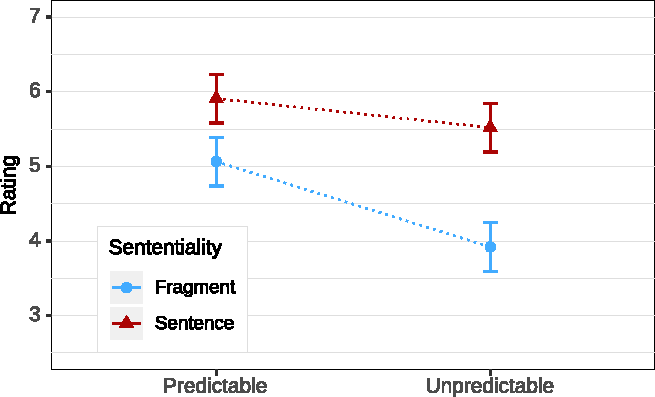
\includegraphics[scale=1]{figures/scr_rating_estimates}
 \caption{Mean ratings $+$ 95\% CIs for experiment \ref{exp:scripts-rating}. \label{fig:scripts-rating-means}}
\end{figure}

The final model contains significant main effects for both experimentally manipulated IVs. The main effect of \textsc{Sententiality} \clmmLR{30.05}{\highsig} reveals a general preference for sentences over fragments, and the main effect of \textsc{Predictability} \clmmLR{10.49}{0.01} shows that predictable utterances are also preferred overall. The significant interaction \clmmLR{9.61}{0.01} between both predictors confirms the prediction of UID\is{Uniform Information Density} that the relative preference for sentences is weaker in the predictable condition: Fragments are more acceptable when they refer to a predictable event. \textsc{ScriptKnowledge} does not seem to constrain this interaction given the model, as the three-way interaction was not significant \clmmLRnonsig{2.36}{0.1}. There is also no significant main effect of \textsc{ScriptKnowledge} \clmmLRnonsig{0.03}{0.8}, but a significant interaction with \textsc{Predictability} \clmmLR{5.08}{0.05}: The more people know about a scenario, the more they distinguish between the predictable and unpredictable conditions. The absence of any significant effect of \textsc{ScriptType} or interaction with other predictors suggests that the situational and adapted instrumental scripts\is{Script knowledge} trigger equally strong predictability effects. Finally, there is a theoretically uninteresting \textsc{Position} main effect that however does not interact with any of the other predictors and shows that ratings improve in the course of the experiment.

\begin{table}[t]
\centering
\caption{Fixed effects in the final CLMM. \label{tab:scripts-rating-estimates}}
\begin{tabular}{p{3.4cm}lllll}
\lsptoprule
Predictor & Estimate & SE & $\chi^2$ &  $p$-value &  \\   
\midrule
\textsc{Sententiality}      &  -0.958 & 0.143 & 30.5 & \textless 0.001 & ***\\
\textsc{Predictability}    &   \phantom{-}0.554 &  0.162 & 10.49 & \textless 0.01 & ** \\
\textsc{ScriptKnowledge}    &  \phantom{-}0.012 &  0.109 & \phantom{1}0.03 & \phantom{\textless }0.86  &  \\
\textsc{Position}   & \phantom{-}0.021 & 0.002 & 21.57 & \textless 0.001 & *** \\
\textsc{Sententiality:}\linebreak \textsc{Predictability} &   \phantom{-}0.22 &  0.073  & \phantom{-}9.61 & \textless 0.01 & **\\
\textsc{Predictability:} \textsc{ScriptKnowledge}   &  \phantom{-}0.206 & 0.094 & \phantom{1}5.08  & \textless 0.05 & *\\
\lspbottomrule
\end{tabular}
\end{table}

\subsection{Discussion}
\label{sec:scripts-rating-discussion}
Experiment \ref{exp:scripts-rating} shows that fragments are more acceptable when they refer to a message that is predictable in context. This shows that the manipulation of utterance predictability through script knowledge\is{Script knowledge} works and that information-theoretic\is{Information theory} considerations determine the preferred form of utterances. 

\subsubsection{Script-based event chains as an approximation to context}
First of all, the experiment confirms the suitability of the script\is{Script knowledge}-based manipulation of predictability, which is empirically founded on event probabilities\is{Event chain} estimated from the DeScript corpus\is{Corpus} of script knowledge\is{Script knowledge} \citep{wanzare.etal2016}. This is evidenced by the main effect of \textsc{Predictability}, which confirms that utterances that refer to predictable events are perceived as more natural across the board. The interaction between \textsc{Predictability} and the \textsc{ScriptKnowledge} scores collected with the questionnaire following the main experiment shows that this effect is particularly strong when subjects are familiar with a scenario. This confirms the utility of the materials as triggers for script\is{Script knowledge}-based expectations.

\subsubsection{Evidence for information-theoretic constraints}

From the information-theoretic\is{Information theory} perspective, the most important result of the experiment is the significant \textsc{Sententiality:Predictability} interaction. As information theory predicts, fragments are more acceptable when they encode a predictable message than when they encode an unpredictable one. Experiment \ref{exp:scripts-rating} thus provides first empirical evidence that the perceived acceptability of a fragment depends on the likelihood of the message they encode. 

It might seem surprising that sentences were rated\is{Acceptability rating task} as more acceptable than fragments across all conditions. Fragments are frequently used, and if informa\-tion-theoretic\is{Information theory} constraints determine the choice of an utterance there must be situations where a fragment is the most well-formed encoding for a message. For most of my materials however, the sentence was also preferred in the predictable condition.%
%
\footnote{In three of the 24 items, the fragment was rated\is{Acceptability rating task} as more acceptable than the sentence in the predictable condition on average. In the unpredictable condition, this was never the case.}\afterfn%
%
Even though this is unexpected, UID\is{Uniform Information Density} does not make predictions about a main effect of \textsc{Sententiality} that could be investigated with experiment \ref{exp:scripts-rating}. UID\is{Uniform Information Density} does also not predict whether the interaction is strong enough to invert a potential preference for fragments or sentences in one of the \textsc{Predictabi\-lity} conditions, and information-theoretic constraints are certainly not the only factor that determines the choice of an encoding. Depending on which other factors are at work in the context of the relatively diverse materials, these can potentially override effects of information-theoretic constraints. Furthermore, as I anticipated above, the script knowledge\is{Script knowledge}-based predictability manipulation that I adopted implies that likely events are more likely to be talked about. Even if this assumption is correct (the production data\is{Production task} collected in experiment \ref{exp:scripts-production} confirm it), quantitative predictions about \textit{how much} more or less well-formed an encoding is can only be made if it is known how likely the corresponding message is. From this perspective, all that the experiment can show, and that it does show, is that predictability has an effect on the acceptability of fragments. Even if the likelihood of a message in the context of my materials is still unknown, the probability that a message is likely enough to license ellipsis will be higher the more likely that event is. 

\subsubsection{Why are sentences more acceptable?}

The observation that sentences are preferred over fragments both in the predictable and the unpredictable conditions is unexpected, even though as I discussed above, this does not challenge the interpretation of the data as evidence for my UID\is{Uniform Information Density}-based account. In what follows I discuss several potential reasons for this preference for sentences: (i) the written presentation modality, (ii) politeness considerations, (iii) pragmatic considerations of the choice for a specific fragment, and (iv), a potential mismatch between the likelihood of an event and that of a corresponding utterance. 

First, the written presentation might yield a preference for sentences, because fragments seem to be less appropriate in written speech. I attempted to counteract this by explicitly presenting the target utterance as spoken by one of the characters, but effects of the written presentation cannot be ruled out. Alternatively, materials could be presented auditorily, but this would increase the complexity of the experiment, because prosody must be controlled.

Second, in some situations the use of fragments might be perceived as too informal. I addressed this issue with a questionnaire on the formality of the script\is{Script knowledge}-based situation underlying my materials which was presented after experiment \ref{exp:scripts-production}. The questionnaire was presented in the same way as the script knowledge\is{Script knowledge} questionnaire presented after experiment \ref{exp:scripts-rating}. Participants used a 5-point Likert scale (5 = very formal) to rate how formal they perceived the situation described by each script\is{Script knowledge}. I then investigated a potential effect of the mean formality rating with linear models, which show that the effect of formality on the relative preference for fragments is far from being significant \lmnonsig{1}{0.26}{0.6}.%
%
\footnote{The IV in the analysis consisted in the mean formality ratings per scenario. The DV was the difference between the mean rating for the sentence and the mean rating for the fragment per scenario. The full model contained only a main effect of \textsc{Formality} and the final model was an intercept-only model. As for previous analyses, models were fit with the \texttt{lme4} package \citep{bates.etal2015} and model comparisons were conducted with the \texttt{anova} function in \texttt{R}.}\afterfn%
%
This suggests that the preference for sentences cannot be attributed to formality.

Third, the average acceptability\is{Acceptability rating task} difference between fragments and sentences might be not due to surprisingly high ratings for sentences, but because some of the fragments were not the optimal encoding in the predictive condition. Recall that in order to control the form of fragments I always tested DP\is{Determiner phrase} fragments that appeared in the postverbal position in the full sentence. This ensured that materials were as similar as possible to each other in length and internal structure, but this type of fragments is not necessarily the most optimal one with respect to UID\is{Uniform Information Density}. As I observed in the introduction to this section, fragments can have different syntactic categories, or consist of a sequence thereof. Therefore, a wide range of fragments can be derived from a single sentence like \Next[a], some of which are given in \Next[b-d]. In the specific case of the pasta scenario, the DP\is{Determiner phrase} \Next[b] might be rather uninformative\is{Shannon information}, because cooking pasta involves various events that concern the pasta. Following UID\is{Uniform Information Density}, in this case, \textit{the pasta} might be omitted due to its predictability rather than the PP\is{Preposition phrase} in \Next[d], which would survive ellipsis because it is less predictable. If that was the case, at least some of the fragments tested in the experiment might not (only) be degraded because a sentence is preferred in the situation, but because there are other fragments that are more well-formed and can communicate the same message.

\ex. \a. Pour the pasta into the pot, please!
\b. The pasta!
\c. The pasta into the pot!
\d. Into the pot!

Finally, the assumption underlying the design of the materials, that a likely event is more likely to be talked about, so far has not been empirically evidenced. As I noted above, information theory\is{Information theory} might even predict the opposite, because referring to an event that follows necessarily from context is extremely redundant.%
%
\footnote{Such considerations also seem to be reflected in the original DeScript data. Some contributors to the corpus\is{Corpus} provide very brief descriptions of the cooking pasta scenario, for instance they omit events like pouring salt into the water or even the action of turning the stove on, which is a necessary condition for events that occur later in the script\is{Script knowledge}.}\afterfn%
%
If the messages in the predictable conditions were not as likely as I assumed them to be, this would also explain the overall preference for sentences. This does not undermine the conclusions that I draw so far from the experiment: If utterances that refer to predictable events were unlikely in the context of my materials, the interaction would be expected to go in the opposite direction. Even if both the fragment and the sentence were highly redundant, UID\is{Uniform Information Density} still predicts that the less redundant fragment will be preferred over the full sentence.%
%
\footnote{\citet{schafer.etalunderreview} present data on verb phrase ellipsis\is{Verb phrase ellipsis} that are in line with this prediction. In a self-paced reading experiment, they find that longer redundant VPs\is{Verb phrase} \Next[a] are read faster than shorter ones \Next[b] (per word). This indicates lower average surprisal\is{Shannon information} on the longer VPs\is{Verb phrase}. Rating data show that realization of the redundant VP\is{Verb phrase} is more degraded in the long condition than in the short one.

\ex. \a. John played football, and Bill \textit{played football}, too.
    \b.  John played football in the backyard of the house, and Bill \textit{played football in the backyard of the house}, too.

}\afterfn%
% 
This calls for an empirical estimation of the message probability in my materials, which is one of the goals of experiment \ref{exp:scripts-production}. Anticipating the results that I discuss in greater detail in Section \ref{sec:scripts-production-results-check}, the message underlying my materials in the predictable condition is indeed more likely (19.1\%) than that in the unpredictable condition (0.4\%). However, there is a large degree of variation between items. For instance, in the train scenario the message used in the predictable condition was produced in 96.6\% of the trials, whereas there were three scenarios for which the target utterance tested in the predictable condition was never produced.

\subsubsection{Summary and outlook}
Taken together, experiment \ref{exp:scripts-rating} shows that fragments are more acceptable when they refer to a message that is predictable in context. This supports my hypothesis that predictable utterances are more likely to be reduced. The overall preference for sentences is unexpected but does not contradict the predictions of information\is{Shannon information} theory. However, this finding is expected both under UID\is{Uniform Information Density} and a source coding\is{Source coding} approach, which predicts a general tendency to assign shorter codes to more likely messages. UID\is{Uniform Information Density} additionally predicts that specifically those words that are more predictable are omitted. This is investigated with a production task\is{Production task} in experiment \ref{exp:scripts-production}. The production data will also show whether the messages tested in the predictable condition are indeed likely more likely than the presumably unpredictable ones.

%%%%%%%%%%%%%%%%%%%%%%%%%%%%%%%%%%%%%%%%%%%%%%%%%%%%%%%
%%%%%%%%%%%%%%%%%% SKRIPTWISSEN PRODUKTION %%%%%%%%%%%%
%%%%%%%%%%%%%%%%%%%%%%%%%%%%%%%%%%%%%%%%%%%%%%%%%%%%%%%
\refstepcounter{expcounter}\label{exp:scripts-production}
\section{Experiment \ref{exp:scripts-production}: Script knowledge, production}  \label{sec:scripts-production}
\subsection{Background}
\label{sec:scripts-production-background}

Experiment \ref{exp:scripts-rating} showed that fragments are relatively more acceptable when they encode predictable messages. Even though this follows from UID\is{Uniform Information Density}, it is also predicted by a source coding\is{Source coding} account that simply assigns shorter codes to more likely messages. Experiment \ref{exp:scripts-production} investigates the two more fine-grained predictions of UID\is{Uniform Information Density} on the word level: First, predictable words are more likely to be omitted, because this avoids troughs in the ID profile\is{Information density}. Second, words that reduce the surprisal\is{Shannon information} of unpredictable following words are more likely to be realized, since this smooths peaks in the ID profile\is{Information density}. Source coding\is{Source coding} predicts an overall densification strategy for predictable utterances, but only UID\is{Uniform Information Density} predicts \textit{which} words are omitted and that channel capacity\is{Channel capacity} limits the densification of utterances. This upper bound will be specifically evidenced by the insertion of redundant material in order to reduce peaks in the ID profile\is{Information density}, which is not predicted by source coding\is{Source coding}.

Investigating these predictions empirically requires (i) a data set that contains such omissions, (ii) to know  which words have been omitted, and (iii) a method to estimate information\is{Shannon information} in the presence of omissions. Following the approach taken by \citet{levy.jaeger2007} and subsequent work, logistic regressions can then be used to test whether information\is{Shannon information}-theoretic\is{Information theory} measures significantly contribute to predicting whether this word has been omitted or not in the data set. In experiment \ref{exp:scripts-production} I collected such a data set with a production tsk using the same stimuli as in experiment \ref{exp:scripts-rating}, which contains about 100 utterances for each of the script-based\is{Script knowledge} stories. This allows me to quantify the likelihood of utterances in the extralinguistic context\is{Context, extralinguistic} modeled by the stories. The data were preprocessed so that omissions can be unambiguously reconstructed. I estimate word probabilities for omitted and realized words in this data set with  a new method of surprisal\is{Shannon information} estimation which is not confounded by omissions in the data.

Experiment \ref{exp:scripts-production} will also provide further insights on the question of whether word order\is{Word order} variation is driven by UID\is{Uniform Information Density}. As I discussed in Section \ref{sec:infotheory-uid}, it has been argued in the literature that the average surprisal\is{Shannon information} of words is lower the more material precedes them in the clause. Therefore, placing unpredictable words in a sentence-final position and predictable ones sentence-initially yields a more uniform ID profile\is{Information density} on average. Finally, the experiment will show whether the utterances in the predictable condition of the rating study\is{Acceptability rating task} were indeed more likely than the unpredictable ones. As I observed in the discussion of experiment \ref{exp:scripts-rating}, likely events are not necessarily likely to be talked about, because the corresponding utterances are rather uninformative\is{Shannon information}.

\subsection{Materials}
I used the context stories of experiment \ref{exp:scripts-rating} as stimuli. These stories consist of four sentences, the first one introduces the script\is{Script knowledge} and the other three ones describe a sequence of three events\is{Event chain} that are likely to follow each other in DeScript. The stimulus corresponding to the pasta script\is{Script knowledge} is given in \Next.%
%
\footnote{I provide English\is{English} translations of the materials in this section, but the experiment was done in German\is{German}.}\afterfn%
% 
In the rating study\is{Acceptability rating task}, the sentence introducing the utterance was always a complete sentence, e.g. \textit{Now Annika says to Jenny}. In the production study\is{Production task} this sentence was replaced by a fragment of the form \textit{$\langle$Person A$\rangle$ to $\langle$Person B$\rangle$}. Otherwise the force of this introduction could have biased participants to produce e.g. declarative or interrogative utterances instead of the overall most likely utterance.

\ex. Annika and Jenny want to cook pasta. Annika put a pot with water on the stove. Then she turned the stove on. After a few minutes, the water started to boil. \\Annika to Jenny: \label{ex:scripts-production-item}

I collected data for the 24 scripts\is{Script knowledge} on which the materials in experiment \ref{exp:scripts-rating} were based. Some of the materials were slightly adapted, so that there were only two characters in each script\is{Script knowledge}. In the rating study\is{Acceptability rating task}, some stories had three participants, for instance, the traveling couple and an airline employee. %

\subsection{Procedure}
The experiment was completed by 198 self-reported native speakers of German\is{German}, who were recruited for the experiment on the \textit{clickworker} crowdsourcing platform. Subjects were paid \currencyEuro{2} for participating in the study. The task consisted in reading the context story and entering the sentence the subject considered most likely into a text field. Initially, I planned to collect two data sets using the same materials, one that contains omissions and one that contains only complete sentences. The nonelliptical data set could then be used for surprisal\is{Shannon information} estimation (without surprisal\is{Shannon information} being affected by omissions) whereas the data set containing omissions would have shown whether word probabilities in the nonelliptical data set predict the actual distribution of omissions. However, even though participants were instructed to produce \textit{complete sentences}, they produced a relatively high ratio of utterances containing omissions. Therefore, I used this data set as the elliptical one and reconstructed ellipses as described in Section \ref{sec:scripts-production-annotation} in order to obtain a nonelliptical data set for probability estimation. In order to rule out the possibility that the term \textit{sentence} in the instructions resulted in an artificially low rate of omissions, I collected a smaller data set ($n$ = 30 for each script) replacing the term \textit{sentence} in the instructions by \textit{utterance}. I then compared the ratio of elliptical utterances, which lacked at least one word that appears obligatorily in a full sentence between both data sets. In the data set collected by asking for \textit{utterances}, the rate of elliptical utterances (25.74\%) was slightly higher than in the data set collected by asking for \textit{sentences} (23.79\%). A linear mixed effects regression on the item level shows that this difference is not significant \clmmLRnonsig{0.8}{0.37}. I conclude that the term \textit{sentence} in the instructions did not bias subjects' behavior as compared to \textit{utterance} and therefore used the larger data set for analysis and reconstructed the nonelliptical data set for analysis.

Subjects were also told that they would read statements like \textit{$\langle$Person A$\rangle$ to $\langle$Person B$\rangle$} after the story, and that these statements specified whose utterance they should produce. Subjects were assigned to one of two lists, and each list was worked on by 99 participants. Each list contained half of the 24 script-based\is{Script knowledge} materials and eigtht further stimuli. These materials had the same form as the script-based\is{Script knowledge} materials (a four-sentence context story), required the same task and also described potentially script-based\is{Script knowledge} situations. However, they were not as based on empirically measured event probabilities. The purpose of including them was to obtain a larger data base for future analyses of omissions in fragments. Materials were presented in fully randomized order. After data collection, subjects were asked to complete a questionnaire on how formal they perceived the situations described in the materials on a 5-point Likert scale (5 = very formal). These data were used as predictor for the post-hoc analysis on formality in the rating study\is{Acceptability rating task} that I reported in the discussion of experiment \ref{sec:scripts-rating}. There were no attention checks, but the data provided by some subjects were excluded because they entered random character strings or copied part of the stimulus into the text field.

\subsection{Preprocessing} \label{sec:scripts-production-annotation}

The raw data set comprised about 100 utterances for each of the 24 items. Subjects produced a diverse set of utterances even for semantically identical or very similar meanings referring to the same event. \Next shows some typical responses for the pasta script\is{Script knowledge}. For instance, the responses vary with respect to lexical alternatives such as the synonyms \textit{Pasta} and \textit{Nudeln} in \Next[a,b], optional adverbials\is{Adverbial} like \textit{jetzt} `now' in \Next[c] and omissions like that of \textit{in den Topf} `into the pot' in \Next[d]. In addition, these utterances vary in word order\is{Word order}, which depends on the insertion of modals as \textit{kannst} `can' in \Next[a--c] that make the indirect speech act more polite and on sentence force, as the difference between declaratives and interrogatives in \Last[c,d] shows.

\ex. \ag. Kannst du die Pasta in den Topf tun?\\
can.\textsc{2sg} you the pasta in the.\textsc{acc} pot do\\
\trans{Can you put the pasta into the pot?}
\bg. Kannst du die Nudeln in den Topf füllen?\\
can.\textsc{2sg} you the noodles in the.\textsc{acc} pot fill\\
\trans{Can you put the pasta into the pot?}
\cg. Wir können jetzt die Nudeln rein tun.\\
we can now the pasta inside do\\
\trans{Now we can put the pasta in.}
\dg. Gibst du die Nudeln rein?\\
give.\textsc{2sg} you the noodles inside\\
\trans{Can you put the pasta in?}

The diversity in the production data\is{Production task} results in two problems that were addressed by preprocessing the data to a standardized form. First, it complicates the resolution of ellipsis, which is necessary in order to investigate whether those words that have been omitted are really more predictable than those which are realized. If there are two synonym lexical alternatives like \textit{Nudeln} and \textit{Pasta}, even if it is obvious that a word referring to \textit{the pasta} is missing, it is unclear which of the alternatives is to be inserted. Second, language models operate on word forms and treat synonyms like \textit{Nudeln} and \textit{Pasta} as distinct expressions. However, if a DP\is{Determiner phrase} referring to the pasta is omitted because of its high predictability, this should be reflected in the information\is{Shannon information} estimated by the language model instead of splitting its probability mass between various synonyms.%
%
\footnote{Higher order \textit{n}-grams\is{N-gram language model} boost this problem further. For instance, only two synonym verbs \textit{reingeben}, \textit{reintun} (`to put inside') and two synonym words for the pasta split the probability mass of \textit{pour pasta} across four bigrams\is{Bigram language model}.}\afterfn%
%

\begin{figure}[t]
\begin{tikzpicture}[scale=1]
\draw [draw = black!20!, line width = .5mm] (0,-.9) rectangle (12,-2.2);
\node (t) at (2.026,-1.16) [fill = black!20!, inner sep = 3pt] {Original production data};
\node (mp) at (5.7,-2){
\begin{minipage}{6cm}
~~
\end{minipage}
\begin{minipage}{.5cm}
 ~~
\end{minipage}
\begin{minipage}{5.5cm}
\texttt{Schnell die Nudeln in den Topf!}\\
\vspace{.4cm}
\end{minipage}

};
%%% CONTENT EXTRACTION
\draw [draw = black!20!, line width = .5mm] (0,-2.7) rectangle (12,-4.9);
\node (t) at (1.247,-2.96) [fill = black!20!, inner sep = 3pt] {Content words};
\node (mp) at (5.7,-4.1){
\begin{minipage}{6cm}
\vspace{-.4cm}
\begin{itemize} \itemsep0em
  \item Annotate  case and prepositions 
 \item Pool synonyms and lemmatize
\end{itemize}
\end{minipage}
\begin{minipage}{.5cm}
 ~~
\end{minipage}
\begin{minipage}{5.5cm}
\texttt{schnell nudeln topf.goal}\\
\vspace{.4cm}
\end{minipage}

};

\draw [draw = black!20!, line width = .5mm] (0,-5.4) rectangle (12,-7.6);
\node (t) at (2.367,-5.66) [fill = black!20!, inner sep = 3pt] {Adjuncts and function words};
\node (mp) at (5.7,-6.8){
\begin{minipage}{6cm}
\vspace{-.4cm}
 \begin{itemize} \itemsep0em
  \item Remove adjuncts and auxiliaries
  \item Remove function words
\end{itemize}
\end{minipage}
\begin{minipage}{.5cm}
 ~~
\end{minipage}
\begin{minipage}{5.5cm}
\texttt{nudeln topf.goal}\\
\vspace{.4cm}
\end{minipage}

};

\draw [draw = black!20!, line width = .5mm] (0,-8.1) rectangle (12,-10.3);
\node (t) at (1.487,-8.36) [fill = black!20!, inner sep = 3pt] {Ellipsis resolution};
\node (mp) at (5.7,-9.5){
\begin{minipage}{6cm}
\vspace{-.4cm}
 \begin{itemize} \itemsep0em
  \item Full verbs
  \item Arguments of full verbs
\end{itemize}
\end{minipage}
\begin{minipage}{.5cm}
 ~~
\end{minipage}
\begin{minipage}{5.5cm}
\texttt{schütten.null nudeln topf.goal}\\
\vspace{.4cm}
\end{minipage}

};
\node at (7.1,-2.7)[single arrow, single arrow head extend=10pt, single arrow tip angle=130, shape border rotate=270,inner sep=8pt, fill=black!20!, minimum height=1.2cm]{~~~~};
\node at (7.1,-5.4)[single arrow, single arrow head extend=10pt, single arrow tip angle=130, shape border rotate=270,inner sep=8pt, fill=black!20!, minimum height=1.2cm]{~~~~};
\node at (7.1,-8.1)[single arrow, single arrow head extend=10pt, single arrow tip angle=130, shape border rotate=270,inner sep=8pt, fill=black!20!, minimum height=1.2cm]{~~~~};

\end{tikzpicture}
\caption{Overview of the preprocessing procedure applied to the production data. First, case and prepositions are annotated on the noun phrases, then the adverb \textit{schnell} is removed and finally the missing verb \textit{schütten} (`to pour') reconstructed.\label{fig:prod-preprocessing}}
\end{figure}
%
Therefore, all utterances produced by the subjects were manually annotated according to a procedure, which is exemplified in Figure \ref{fig:prod-preprocessing} and which transforms an utterance like \Next[a] into an abstract representation \Next[b]. Overall, preprocessing consisted in a trade-off between the necessary standardization and the preservation of as much variation in the original data as possible. Specifically, preprocessing preserved word order\is{Word order} and morphosyntactic properties of noun phrases\is{Noun phrase}, such as distinctive case inflections, which provide a cue toward the \texttheta-role of the noun in fragments. The standardization consisted in pooling synonyms and removing adjuncts\is{Adjunct}, adverbials\is{Adverbial} and function words. Finally, I also annotated representations of the meaning of each utterance. This annotation layer is necessary to investigate whether more predictable meanings are assigned shorter codes and to relate the production data\is{Production task} to the rating data\is{Acceptability rating task} from experiment \ref{exp:scripts-rating}.

\ex. \ag. Schnell die Nudeln in den Topf!\\
	  quickly the pasta in the pot\\
	  \trans{(Pour) the pasta quickly into the pot!}
     \bg. \texttt{schütten.\textsc{null}} \texttt{nudeln} \texttt{topf.\textsc{goal}}\\
	pour.\textsc{null} pasta pot.\textsc{goal}\\

\subsubsection{Exclusion of noisy data}
Before preprocessing, data that were clearly not meaningful utterances in the situation described in the stimulus were removed from the data set. This concerns data from two subjects who provided responses in English\is{English}, responses consisting in random character strings, copied and pasted parts of the stimulus material or nonsense utterances. For instance, one subject repeatedly entered `hello', even in scripts\is{Script knowledge} where it was unnatural that one of the characters would greet the other one. Utterances that corresponded to wrong turns (e.g. by the customer in the library script, where subjects were asked to provide an utterance by the librarian) were also excluded. This resulted in a loss of 8.82\% of the responses. Sometimes subjects provided two or more utterances in a single trial, such as the example in \Next. In such cases, both utterances were separated and treated as individual utterances by the same subject. Separation occurred when two matrix sentences were separated by punctuation characters.

\exg. Gibst du mir bitte die Nudeln? Das Wasser kocht.\\
      give.\textsc{2sg} you me.\textsc{dat} please the noodles the water boils\\
      \trans{Would you give me the pasta, please? The water is boiling.}

\subsubsection{Annotation of content words}

All utterances were transformed into representations that contain the matrix verb and its arguments. In the complete data from a script, i.e. item, all coreferent nouns were pooled to the same lemma, for instance \textit{Pasta} and \textit{Nudeln} were merged to \texttt{nudeln}. Among the synonyms, the most frequent one was chosen as a label. The same procedure was applied to synonym verbs, such as \textit{schütten} `pour', \textit{füllen} `fill', \textit{reingeben} `put inside' and \textit{reintun} `put inside' in \LLast, which were merged to \texttt{schütten} `pour'. Some verbs are ambiguous, for instance, \textit{geben} can be used either as a part of a particle verb \textit{reingeben} `put inside', like in \LLast[d], but it can also describe a transfer of possession `give' as in \Last. Therefore, only the instances of \textit{geben} belonging to the particle verb were pooled to \texttt{schütten}. Pronouns were also resolved and pooled to the corresponding noun lemma.

For all nouns, distinctive case morphology was annotated as a suffix $.\langle$\textsc{case}$\rangle$ attached to the noun to ensure that the language model treated nouns with differential case marking (but only those) as different items. This is relevant because experiments \ref{exp:case}--\ref{exp:scripts-rating-case} provided evidence for case connectivity\is{Case connectivity}: A DP\is{Determiner phrase} fragment appears in the same case as the DP\is{Determiner phrase} in the corresponding full sentence does. From the hearer's perspective, case can thus be a strong cue toward a specific complete sentence. For instance, a dative\is{Dative case} DP\is{Determiner phrase} fragment excludes all possible interpretations that require it to appear in accusative\is{Accusative case}. Case was annotated only when it was morphologically distinguished, because otherwise it does not function as such a cue. Similarly, prepositions were annotated as a suffix $.\langle$\textsc{preposition}$\rangle$ attached to the noun, because the experiments on preposition omission\is{Preposition omission} in German\is{German} showed that there is a strong tendency not to omit prepositions\is{Preposition omission} in PPs\is{Preposition phrase} in German\is{German}.

\subsubsection{Removal of function words, adverbials and auxiliaries}
After the annotation of case and preposition information on nouns, all function words, like articles and prepositions, modal verbs and auxiliaries as well as optional words like adjuncts\is{Adjunct} were removed from the data set. As for function words, the reason for this is that articles\is{Article omission} and prepositions\is{Preposition omission} cannot be freely omitted in German\is{German}: Article omission\is{Article omission} is not grammatical in standard German\is{German} but only in specific text types \citep{reich2011, reich2017}, and my experiment \ref{exp:pstranding-german} showed that the omission of prepositions\is{Preposition omission} is heavily degraded. Since the purpose of collecting this data set is to investigate omissions on the word level, treating e.g. a preposition\is{Preposition phrase} and its complement DP\is{Determiner phrase} as two separate units would falsely suggest that they can be omitted independently from each other. Adverbials\is{Adverbial} can be inserted relatively freely at various positions of the sentence in German\is{German} \citep[209]{eisenberg1999}, but often the information\is{Shannon information} that they convey, such as time, place or manner is left implicit. Therefore, it is not reasonable to assume that e.g. \Next involves ellipsis of a temporal and a locative adverbial \citep[1850]{reich2011}. 

\ex. $\langle$Yesterday evening$\rangle$ John ate a pizza $\langle$at Giordano's$\rangle$.

Of course, the aspects of meaning contributed by adverbials\is{Adverbial} might be also subject to UID\is{Uniform Information Density}: If John eats at Giordano's frequently, the adverbial \textit{at Giordano's} will be less informative\is{Shannon information} and therefore more likely to be omitted than if he does only rarely. However, omitting the adverbial does not yield a fragment under any theoretical account, therefore the omission of such optional expressions is not directly relevant to my research questions.

Modal verbs and auxiliaries can affect word order\is{Word order} in German\is{German}. Specifically in questions which are used as indirect speech acts, the modal verb occurs in the sentence-initial matrix verb position and the main verb utterance-finally \Next[a]. In declaratives, modals occupy the default left bracket position \Next[b]. In order to keep the annotation procedure simple I omitted any occurring modals, but left the main verb in the final position where it appears in the original data. Maintaining the original word order\is{Word order} as much as possible is necessary in order to take into account effects of word order\is{Word order} on information\is{Shannon information}. Utterance-final words can be predicted from preceding material \citep{levy2008}%
%
\footnote{But see \citet{balling.kizach2017} for conflicting results on Danish\is{Danish}.}\afterfn%
%
and will therefore be on average less informative\is{Shannon information} than sentence-initial ones.

\ex. \ag. Kannst du die Nudeln in den Topf füllen?\\
can.\textsc{2sg} you the noodles in the.\textsc{acc} pot fill\\
\trans{Could you fill the pasta into the pot?}
\bg. Du könntest schon mal die Teller auf den Tisch stellen.\\
you can.\textsc{sbjv.2sg} already \textsc{prt} the plates on the table put\\
\trans{You could now put the plates on the table.}

\subsubsection{Ellipsis resolution}

In order to estimate (and to later compare) the surprisal\is{Shannon information} of realized and originally omitted words, all ellipses, i.e. omissions of words that are obligatory in full sentences, were reconstructed. This involved specifically the insertion of omitted main verbs and arguments. Note that the set of ellipses in the data encompasses not only those omissions that yield fragments according to the definition provided in Section \ref{sec:intro-fragments}, but also argument omissions. Testing whether omissions of individual words are in line with the predictions of UID\is{Uniform Information Density} requires not only to compare fragments and complete sentences, but to take into account also the possibility of other argument ellipses, like topic\is{Topic drop} or object drop\is{Object drop}.

\begin{sloppypar}
Ellipses could in general be unambiguously resolved, because the reconstruction procedure operated on the preprocessed simplified representations described above and there were no lexical alternatives to choose from. If there were several possibilities of enriching a fragment, the strategy that required the least amount of insertions and default subject-initial word order\is{Word order} was pursued. All words inserted during this procedure received an additional tag \texttt{.NULL}, which indicated that they had been omitted in the utterances produced by the subjects. The purpose of the tag was to keep track of which words had been omitted and which ones had been realized in the original data set. In the statistical analysis, I used this binary \textsc{Omission} predictor as the dependent variable.\end{sloppypar}

Based on the annotated data, I created two versions of the data set: The \textit{original} data set, where I kept track of actual omissions, and the \textit{enriched} data set, which was used only for the purpose of surprisal\is{Shannon information} estimation. This data set contains all of the originally produced words and those that had been inserted through ellipsis reconstruction. I removed the \texttt{.NULL} tags assigned to reconstructed words from the words in this data set, since otherwise the reconstructed and realized occurrences of the same word would be treated as different lexicon entries during surprisal\is{Shannon information} calculation. Using a data set without omissions for surprisal\is{Shannon information} estimation addresses a central problem of language modeling on elliptical data: If UID\is{Uniform Information Density} is correct, word probabilities estimated from a regular corpus\is{Corpus} are not proportional to the likelihood of these words. Since speakers omit predictable words more often, they are expected to be rare in the corpus\is{Corpus}, or at least not as frequent as they would be without omissions. Therefore, word probabilities estimated from a regular corpus\is{Corpus} are not proportional to the likelihood of these words. This circularity issue, which is discussed in detail below in Section \ref{sec:scripts-production-surprisal-context}, does not arise in data sets which do not contain any omissions.

\subsubsection{Annotation of messages}
Finally, the meaning of each utterance was annotated as a simplified semantic representation consisting of a verb and its arguments. These representations were formally identical to those in the enriched data set, but insensitive to word order\is{Word order}. The rationale was to assign the same single label to all meaning-equivalent expressions. The purpose of this annotation layer was to be able to quantify the likelihood of meanings and to model the mapping from signals (i.e., utterances) to messages. In this case this mapping was unidirectional, so that various signals could refer to the same message, but not \textit{vice versa}. In principle the opposite would also be possible, but there were no ambiguous utterances in the context of the tightly constrained script-based\is{Script knowledge} stories. 

\subsection{Surprisal estimation}
\label{sec:scripts-production-surprisal}

I argued above that reasonably estimating the surprisal\is{Shannon information} of words in fragments is possible as long as effects of extralinguistic context\is{Context, extralinguistic} can be taken into account and it is known which words have been omitted. The data set whose collection and preprocessing is described in the preceding section conforms to both of these needs. The contexts\is{Context, extralinguistic} used for data elicitation ensure that the probabilities of words and utterances in the data set are conditioned on these contexts. The reconstruction of ellipsis solves the circularity issue that might arise from the frequent omission of predictable words: Surprisal can be estimated from the enriched data, which includes words that have originally been omitted and is consequently not increased by their more frequent omission.

I explore effects of three information-theoretic\is{Information theory} predictors on omissions. In order to take the script-based\is{Script knowledge} approximation to extralinguistic context\is{Context, extralinguistic} into account, I apply all methods separately to the data for each script\is{Script knowledge}. The first method that I use is simply unigram\is{Unigram language model} surprisal\is{Shannon information}. Since the language models are trained on the data for each script\is{Script knowledge} separately, unigram\is{Unigram language model} surprisal\is{Shannon information} models extralinguistic context\is{Context, extralinguistic}. This contrasts with unigram\is{Unigram language model} surprisal\is{Shannon information} estimated from larger and more balanced corpora\is{Corpus}, where the frequency of a word is not conditional on a tightly controlled context. The second method that is an extension of the calculation of surprisal\is{Shannon information} suggested by \citet{hale2001}. In addition to extralinguistic context\is{Context, extralinguistic}, this method also takes linguistic context\is{Context, linguistic} into account, and unlike \citeauthor{hale2001}'s original method, it can deal with the possibility of arbitrary omissions in fragments. These two surprisal\is{Shannon information} measures will show whether predictable words are more likely to be omitted. I interpret this as the result of a strategy to avoid troughs in the ID profile\is{Information density}. Finally, I use a measure of surprisal\is{Shannon information} reduction, which is technically similar to context-dependent surprisal\is{Shannon information}, in order to investigate to what extent non-final words reduce the surprisal\is{Shannon information} of the following word. This could provide evidence for a strategy to avoid peaks in the ID profile\is{Information density}.

\subsubsection{Unigram surprisal}

Unigram language models\is{Unigram language model} with Good-Turing discount were trained on the enriched data ($n \sim 100$) for each script\is{Script knowledge} using the SRILM toolkit \citep{stolcke2002}. I estimated unigram surprisal\is{Shannon information} for each script\is{Script knowledge} independently. This method allows for the interpretation of the probability estimate $S(w_i) = -\log_2\;p(w_i)$ for a word $w_i$ as the probability of $w_i$  given extralinguistic context\is{Context, extralinguistic}, which is set by the context story, i.e. $S(w_i) = -\log_2\;p(w_i\mathbin{|} context_{extraling.})$. The by-word unigram surprisal\is{Shannon information} values were then extracted from the language model files and annotated with Python scripts for each word in the production data. 

\subsubsection{Taking linguistic context into account}
\label{sec:scripts-production-surprisal-context}

In previous studies on predictability effects on linguistic encoding preferences, the probability of words in context has been estimated with \textit{n}-gram language models\is{N-gram language model}. As I anticipated above, training \textit{n}-gram models on corpora that contain elliptical data results in a circularity issue: If predictable words are more often omitted, they will appear to be rare in the corpus\is{Corpus} just because of their expected high rate of predictability-driven omission. 

In the case of unigram\is{Unigram language model} surprisal\is{Shannon information}, this issue can be addressed by training the models on the enriched data set, where all ellipses have been reconstructed. Since there are no omissions in the data, all surprisal\is{Shannon information} estimates reflect the true probability of a target word. However, training higher order \textit{n}-grams\is{N-gram language model} on the enriched data set would result in a further issue, because now words that have been originally omitted would be included in the context of a target word and consequently modulate its probability. This is of course highly implausible, because omitted words are not available to the hearer and therefore cannot contribute to this probability. For instance, if somebody uttered the fragment \Next[a] in the pasta scenario, the corresponding structure in the enriched data set would be \Next[b]. A regular bigram model\is{Bigram language model} trained on the enriched data estimates the surprisal\is{Shannon information} of the DP\is{Determiner phrase} fragment as $S_{pasta} = -\log_2 p(pasta\mathbin{|}pour)$. If the verb increases the likelihood of objects that can be poured in this context\is{Context, linguistic}, the surprisal\is{Shannon information} of pasta would be underestimated in comparison to its true value in a discourse-initial\is{Fragment, discourse-initial} fragment like \Next[a].%
%
\footnote{In the literature on grammatical function words, studies investigating effects of a function word's predictability on its own omission (avoid troughs) have used the likelihood of the construction marked by the function word, like a relative  or complement clause\is{Complement clause}, as an approximation to the function word's surprisal\is{Shannon information} \citep{levy.jaeger2007, jaeger2010}. In an analysis investigating whether redundant relative pronouns are inserted before unpredictable target words, \citet{levy.jaeger2007} train their models on a modified version of the corpus\is{Corpus}, from which all relative pronouns have been removed. Therefore, relative pronoun omissions do not affect the estimated surprisal\is{Shannon information} of the target word. Obviously both approaches cannot be applied to fragments, because omissions can target any word in my preprocessed data set.}\afterfn%
%

\ex. \a. The pasta, please!  \label{ex:scripts-production-hale-frag}
     \b. \texttt{pour} \texttt{pasta} \texttt{pot.GOAL} \label{ex:scripts-production-hale-act}

Therefore, I estimated surprisal\is{Shannon information} with a method based on the approach suggested by \citet{hale2001}. \citeauthor{hale2001} derives surprisal\is{Shannon information} from a parallel parser\is{Parser, parallel}\is{Parser, human} that computes all possible parses and rejects those parses that are incompatible with the current input. The set of possible parses is correspondingly updated after processing each word. One of \citeauthor{hale2001}'s main insights is that the amount of work done by the parser\is{Parser, human} is proportional to the total probability mass of the rejected parses: The higher this probability mass is, the more informative\is{Shannon information} is a word.

\is{Parser, parallel|(}This method requires knowing (i) which parses are possible in a situation and (ii) how likely each parse is. \citet{hale2001} obtains both of these measures from a probabilistic context-free grammar (PCFG\is{Context-free grammar}), which comprises a set of re-write rules whose likelihood can be estimated from a corpus\is{Corpus}. The likelihood of a parse is calculated as the product of the probabilities of the individual rules that are required to generate that parse.\is{Parser, parallel|)} Instead of using PCFG\is{Context-free grammar}s, I assume that my enriched production data\is{Production task} set shows which complete structures are possible in that situation and how likely they are. This approach restricts the set of possible parses to those that actually have been produced and therefore excludes pragmatically odd ones, like \Next. In contrast, a PCFG\is{Context-free grammar} does not exclude odd utterances if they can be derived by its rules. If there is a rule \NNext[a] in the PCFG\is{Context-free grammar}, the unlikely \Next and the likely \Last[b] differ only in the likelihood of the two rules in \NNext, because the other rules required to generate both utterances are identical. Therefore, a PCFG\is{Context-free grammar} could assign a relatively high probability to utterances that are unexpected for pragmatic reasons as compared to a human hearer, who would not expect a request to pour the salt on the table. It seems more psychologically realistic to assume that when a speaker parses\is{Parser, human} the word \textit{pour} and \textit{salt}, the likelihood of \texttt{table.GOAL} as compared to \texttt{pot.GOAL} is not only subject to the likelihood of the re-write rules in \NNext but to a particular context for which a PCFG\is{Context-free grammar} does not account. 

\ex. \texttt{pour} \texttt{salt} \texttt{table.GOAL}

\ex. \a. PP\is{Preposition phrase} $\rightarrow$ \texttt{table.GOAL}
     \b. PP\is{Preposition phrase} $\rightarrow$ \texttt{pot.GOAL}

Therefore, I take the set of unique produced utterances in the enriched data set to represent the range of possible structures and their frequency in the data set to reflect their likelihood in the context of the story. For instance, the German\is{German} equivalent to \ref{ex:scripts-production-hale-act} occurs 16 times among the 115 utterances of the pasta data set, so its likelihood is 0.139. Note that this figure does not represent the likelihood of a sentence equivalent to \ref{ex:scripts-production-hale-act} to be actually produced, because it has been calculated based on the enriched data set and not based on the original production data\is{Production task} that contain omissions, but the likelihood of an utterance that, if it is enriched, corresponds to this representation. Knowing the range of possible structures and their respective probabilities is necessary for the estimation of by-word information\is{Shannon information}.

\is{Parser, parallel|(}Given this general setup, \citet{hale2001} defines surprisal\is{Shannon information} as the logarithm of the ratio of the prefix probability \textalpha, i.e. the probability mass of the parses that are compatible with an input \textit{before} parsing that word to the probability mass of the parses that remain active \textit{after} processing it:

\begin{equation}
 \displaystyle S(w_n) = \log_2 \frac{\alpha_{n-1}}{\alpha_n}
\end{equation}

This measure increases the more $w_i$ narrows the set of parses that are compatible with the input as compared to $\alpha_{n-1}$. If $w_i$ is compatible with all parses that $w_{i-1}$ is compatible with, it equals 0. In the case of utterance-initial words, surprisal\is{Shannon information} is thus equivalent to the negative logarithm of the cumulated probability of all parses (that is, enriched complete structures) that begin with this word.  For illustration, consider the case of an utterance like \Next[a] in the artificial example in \Next, where there are only the four parses in \Next[a--d].

\ex. \label{ex:contexts-pd} \a. \texttt{pour} \texttt{pasta} \texttt{pot.GOAL} \hfill $p = 0.75$\label{ex:contexts-a}
 \b. \texttt{pour} \texttt{salt} \texttt{pot.GOAL} \hfill $p = 0.2$\label{ex:contexts-b}
 \c. \texttt{set} \texttt{table} \hfill $p = 0.03$\label{ex:contexts-c}
 \d. \texttt{pour} \texttt{sauce} \texttt{pan.GOAL}\hfill  $p = 0.02$\label{ex:contexts-d}
 
In this situation, processing \texttt{pour} excludes only the parse in \Last[c], so that $\alpha_{n} = 0.97$. The prefix probability before parsing \texttt{pour}, $\alpha_{n-1} = 1$, because before processing any input no parse is excluded. The surprisal\is{Shannon information} of \texttt{pour} is thus calculated as shown in Equation \ref{eq:surprisal-pour}.

\begin{equation}
 \displaystyle S(pour) = \log_2(\frac{1}{0.97}) = 0.04 \label{eq:surprisal-pour}
\end{equation}

The surprisal\is{Shannon information} of \textit{pasta} after processing \textit{pour} is calculated as shown in Equation \ref{eq:surprisal-pasta}. Since \Last[c] has been previously discarded by processing \texttt{pour}, $\alpha_{n-1} = 0.97$. Processing \texttt{pasta} additionally excludes \Last[b] and \Last[d], so that $\alpha_{n-1} = 0.75$.

\begin{equation}
 \displaystyle S(pasta\mathbin{|}pour) = \log_2(\frac{0.97}{0.75}) = 0.37 \label{eq:surprisal-pasta}
\end{equation}
\is{Parser, parallel|)}

\subsubsection{Accounting for omissions in fragments}     

This method cannot be applied as-is to fragments. For instance, given the discussion on the syntax of fragments in Chapter \ref{sec:chapter-experiments-syntax}, it is possible to encode \Last[a] with the fragment in \Next. However, following the method proposed by \citet{hale2001}, as soon as the parser\is{Parser, human} processes \texttt{pasta} at all, it rejects all of the parses in \Last, because none of them starts with \texttt{pasta}. 

\ex. The pasta!

Therefore, I propose to extend \citeauthor{hale2001}'s method by allowing for an arbitrary number of omissions to occur before and after each word. Checking whether a parse is compatible with an input now does not require for the input to exactly match the parse, starting from its onset, but that the input could have been derived by ellipsis from the parse. For instance, the fragment in \Last can only be derived from \LLast[a] by omitting \texttt{pour} (and \texttt{pot.GOAL}, but this does not matter for estimating the surprisal\is{Shannon information} of \texttt{pasta}). Processing \texttt{pasta} thus excludes the parses in \LLast[b-d], which do not contain this expression. The surprisal\is{Shannon information} of \texttt{pasta} can then be calculated from the total probability mass of these parses by comparing the prefix probabilities as shown in Equation \ref{eq:pasta-s}:

\begin{equation}
S(pasta) = \log_2 (\frac{1}{0.75}) = 0.42 \label{eq:pasta-s}
\end{equation}

This simple modification of \citeauthor{hale2001}'s approach allows in the same way to estimate the surprisal\is{Shannon information} of omitted and realized words in more complex discontinuous fragments. For instance, consider the case of a fragment like \Next, for which by-word surprisal\is{Shannon information} is to be estimated given the probability distribution in \ref{ex:contexts-pd}. The surprisal\is{Shannon information} of \texttt{pour} is calculated as described in the previous paragraph based on the exclusion of \LLast[c] only. The surprisal\is{Shannon information} of the omitted \texttt{pasta} in the context of \texttt{pour} is calculated just like described above for that of the realized word \texttt{pasta}. Note that for the purpose of surprisal\is{Shannon information} estimation it does not matter whether the target word itself has been omitted. This is desirable, since a word's surprisal must be independent from its own omission.

\ex. \texttt{pour} \texttt{pasta.NULL} \texttt{pot.GOAL}

The surprisal\is{Shannon information} of \texttt{pot.GOAL} given \texttt{pour} is then equivalent to the probability mass of the parses that have not been excluded after processing \texttt{pour} but are so after processing \texttt{pot.GOAL}. Since only \Last[d] is excluded by \texttt{pot.GOAL}, this yields a surprisal\is{Shannon information} of 0.03 bits. Unlike it would in an \textit{n}-gram model\is{N-gram language model} trained on the enriched data set, the omitted word \texttt{pasta} does not contribute to the surprisal\is{Shannon information} of \texttt{pot.GOAL} in the example:

\begin{equation}
S(pot.GOAL\mathbin{|}pour) = \log_2(\frac{0.97}{0.95}) = 0.03
\end{equation}

This method avoids the circularity issues related to training language models on elliptical data discussed above. On the one hand, since the complete structures from which the probabilities are derived do not contain omissions, a target word's surprisal\is{Shannon information} is not affect by the actual frequency of its omission. On the other hand, only words that have been actually produced are included in the context of the target word and can affect its probability. This avoids the concern that \textit{n}-gram models\is{N-gram language model} trained on the enriched data falsely include these words in the context. Like the approach by \citet{hale2001}, the approach is fully incremental, because processing effort\is{Processing effort}, i.e. surprisal\is{Shannon information}, arises exactly at the word that triggers the rejection of a parse. By allowing for omissions between words, my approach is similar to skip-gram models\is{Skip-gram language model} \citep{jans.etal2012}. However, unlike a skip-gram model, it does not skip a fixed number of words but take into account the possibility that words \textit{could} have been omitted. A further benefit is that this approach considers as much context as possible, unlike \textit{n}-gram models\is{N-gram language model}. The method presented here covers the complete context, that is, the contextual information about the point in the script\is{Script knowledge} at which the utterance occurs and all material that precedes this word within the utterance.

Although my method relies on the same reasoning as the approach in \citet{hale2001}, the surprisal\is{Shannon information} estimates that its output is mathematically not fully equivalent to Shannon information\is{Shannon information}, because the probabilities of all words that could follow $w_{i-1}$ do not sum to 1.%
%
\footnote{I thank an anonymous CUNY 2020 reviewer for pointing this out.}\afterfn%
%
The reason for this is that in \citeauthor{hale2001}'s approach each parse contributes only to the probability mass of a single word within the set of words $w_i$ that might follow $w_{i-1}$. In order to account for the possibility that a word $w_{i}$ is omitted in the actually produced string, I take also words occurring later in the parse ($w_{i+n}, n \geqq 0$) into account in order to calculate $\alpha_i$. Therefore, a single parse can contribute to the probability mass of two or more words, so the sum of the probability mass of all words in context of $w_{i+1}$ becomes larger than 1. A possibility of dealing with this is to scale $\alpha_i$ by dividing it by the sum of the prefix probabilities of all words $W_{Alt}$ that could follow $w_{i-1}$, as shown in Equation \ref{eq:hale-s-alt}. Scaling ensures that all word probabilities sum to 1.

\begin{equation}
\displaystyle S_{scaled} = \log_2 \frac{\alpha_{i-1}}{\alpha_i \times \sum_{x\in W_{Alt}}{\alpha_x}} \label{eq:hale-s-alt}
\end{equation}

This equation returns a surprisal\is{Shannon information} estimate based on the likelihood of encountering a word at some point after $w_{i-1}$ in the utterance. In that sense, it is similar to unigram\is{Unigram language model} surprisal\is{Shannon information}, the main difference being that previous linguistic context\is{Context, linguistic} restricts the set based on which surprisal\is{Shannon information} is calculated. The problem with this approach however is that it does not model the work done by the parser\is{Parser, human} appropriately: In a situation where a target word is included in all parses, my approach sketched above assigns a surprisal\is{Shannon information} of 0 to this word, because processing it does not result in the exclusion of any of the parses. From a theoretical perspective, this is desirable, because it models proportionality between the work done by the parser\is{Parser, human} and surprisal\is{Shannon information} that underlies the approach in \citet{hale2001}. This property however is lost by scaling the ratio between the prefix probabilities before log-transformation, because if numerator and denominator in Equation \ref{eq:hale-s-alt} differ, the resulting surprisal\is{Shannon information} estimate will never be 0 (except for the rare case that $w_i$ is the only element in $W_{Alt}$). For this reason, I do not scale the prefix probabilities and follow the approach described above instead.

I implemented this surprisal\is{Shannon information} estimation method by first calculating the probability of each of the enriched representations given the complete data set for each script\is{Script knowledge}. I then used these data to calculate the surprisal\is{Shannon information} of each word $w_i$, be it omitted or realized, in the enriched data set by calculating the ratio of the total probability mass of parses compatible with $w_i$ and the preceding $w_{i-1}$. Whether a parse is compatible with an input was tested using regular expressions in \texttt{R}. These regular expressions contained the relevant word(s) and allow for an optional arbitrary number of characters to occur before, after and between each of them, as is indicated by the gaps (\dots) in \Next. %

\ex.\texttt{pour} \texttt{pot.GOAL}
\a. (\dots) \texttt{pour} (\dots)
\b. (\dots) \texttt{pour} (\dots) \texttt{pot.GOAL} (\dots)

The total probability mass of all parses that are compatible with each of these expressions yields the prefix probability $\alpha$ of the last word within this expression. In case of \Last[a], it is calculated by summing up the probabilities of all parses that contain \texttt{pour}, and \Last[b] selects all parses that contain \texttt{pour} and \texttt{pot.GOAL} somewhere later in the parse. These prefix probabilities are then used to calculate by-word surprisal\is{Shannon information}, as sketched above.

Taken together, this approach is fully incremental, applies to fragments and complete sentences alike, allows for arbitrary gaps before, between and after words in fragments, covers the complete linguistic context\is{Context, linguistic} and still assigns a psychologically realistic surprisal\is{Shannon information} estimate to each word within that fragment. However, it requires a set of utterances for which context is tightly controlled and to unambiguously resolve ellipses, therefore it cannot be straightforwardly applied to larger corpora\is{Corpus} that have not been preprocessed in the same way.

\subsubsection{Estimating the reduction of information peaks}
The approximations to surprisal\is{Shannon information} discussed so far are useful to predict the omission of a target word itself, that is, the tendency to omit predictable material. However, UID\is{Uniform Information Density} predicts not only that the surprisal\is{Shannon information} of a word $w_i$ determines the omission of this word. The surprisal\is{Shannon information} of the next word, $w_{i+1}$ also constrains the omission of $w_i$, because inserting $w_i$ before $w_{i+1}$ can reduce a peak in the ID profile\is{Information density} caused by $w_{i+1}$, but only if this insertion makes $w_{i+1}$ more predictable. Examples for this line of reasoning are the insertion of relative pronouns before unexpected RC onsets \citep{levy.jaeger2007} or that of articles\is{Article omission} before unpredictable nouns \citep{lemke.etal2017}. In previous work, this was investigated by including the surprisal\is{Shannon information} of $w_{i+1}$ as a predictor in the analysis. In order to avoid the circularity issue discussed above, this surprisal\is{Shannon information} was not estimated on the original data, but on a version of the data from which all instances of the function word in question, e.g. all articles or relative pronouns, had been previously removed. However, in the case of my data set, all words in the preprocessed data can be omitted, so that removing all potential targets of omission from the data is not an option. Furthermore, UID\is{Uniform Information Density} predicts specifically that redundancy is inserted in order to reduce peaks in the ID profile\is{Information density} and not that any redundant expression is inserted before unpredictable words. If the insertion of a redundant $w_i$ does not reduce $S(w_{i+1})$, it might actually yield a trough in the profile in addition to the following peak and thus yield an even less uniform and efficient use of the channel.

Therefore, instead of using the surprisal\is{Shannon information} of $w_{i+1}$ as a predictor for the insertion of $w_i$, I quantify the effect of the insertion on processing by comparing the prefix probability after processing $w_{i+1}$ when $w_i$ has been inserted to the prefix probability at $w_{i+1}$ in case $w_i$ is omitted:

\begin{equation} 
 \displaystyle Reduction(w_i, w_{i+1}) = \log_2 \frac{\alpha_{w_{i+i}}}{\alpha_{w_i, w_{i+1}}} \label{eq:sreduction}
\end{equation}

If the insertion of $w_i$ does not change the probability distribution after processing $w_{i+1}$, this will result in a reduction of 0. Surprisal\is{Shannon information} reduction is larger the more parses that are compatible with previous context and $w_{i+1}$ are excluded by the insertion of $w_i$. To illustrate how this formula is applied, consider again the omission of \texttt{pasta} in the utterance \texttt{pour} \texttt{pasta.NULL} \texttt{pot.GOAL} in \LLast. If \texttt{pasta} is inserted, only the parse in \ref{ex:contexts-a} is compatible with the input, whereas both \ref{ex:contexts-a} and \ref{ex:contexts-b} are when \texttt{pasta} is inserted. Equation \ref{eq:sreduction} can then be applied to estimate how much inserting \texttt{pasta} reduces the surprisal\is{Shannon information} of \texttt{pot.GOAL}.

\begin{equation} 
 \displaystyle Reduction(pasta, pot.GOAL) = \log_2 \frac{0.97}{0.75} = 0.34
\end{equation}

In contrast to just using the surprisal\is{Shannon information} of $w_{i+1}$ as a predictor of the omission of $w_i$, this method quantifies \textit{how much} the insertion of $w_i$ reduces the surprisal\is{Shannon information} of $w_{i+1}$,  instead of just stipulating that it always does. Therefore, this measure will only predict insertion when this results in a reduction of information\is{Shannon information} on $w_{i+1}$, and not just because the $w_{i+1}$ is overall unpredictable. 

\subsection{Results}
\label{sec:scripts-production-results}

Experiment \ref{exp:scripts-production} had the goal to test the prediction of UID\is{Uniform Information Density} that omissions are distributed so as to reduce peaks and troughs in the ID profile\is{Information density} at the case of a data set collected with a production task\is{Production task}. Given the three surprisal\is{Shannon information} measures discussed in the preceding section, this implies that a higher \textsc{Unigram\is{Unigram language model}Surprisal} and a higher \textsc{ContextSurprisal} increase the likelihood of overtly realizing a word because this avoids troughs in the ID profile\is{Information density}. Inserting words that reduce the surprisal\is{Shannon information} of the following word, that is, words with a high \textsc{SurprisalReduction}, reduces peaks. Furthermore, the data will allow for the investigation of word order\is{Word order} effects predicted by UID\is{Uniform Information Density}, that is, whether predictable words tend toward being placed at the beginning and unpredictable ones at the end of the utterance. The experiment will also show whether predictable events in experiment \ref{exp:scripts-rating} are indeed more likely to be talked about than unpredictable ones.


\subsubsection{Data set}
\label{sec:scripts-production-results-dataset}
The final data set contained about 100 utterances for each of the 24 scripts\is{Script knowledge}. This results in 2.409 utterances and 6.816 primitive expressions that I term ``words'' in what follows. 1,052 words (15.43\% of the total) had been omitted in the original data and were inserted during ellipsis resolution and 561 (23.29\%) of the utterances contained at least one omission. Recall that this comprises both fragments as defined in section \ref{sec:intro-fragments} and argument omissions.

\subsubsection{Distribution of omissions across scripts}

\begin{figure}[t]
 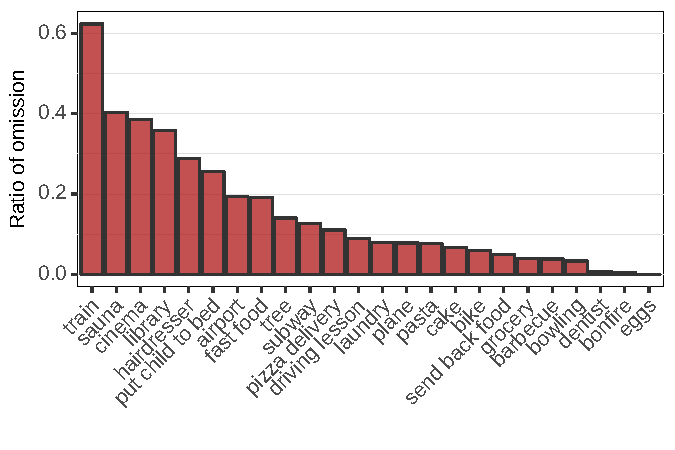
\includegraphics{figures/scr_production_omission_ratio}
 \caption{Ratio of omission across scripts.\label{fig:scripts-ellratio}}
\end{figure}
%
Figure \ref{fig:scripts-ellratio} shows that scripts differ with respect to the ratio of omitted grammatically required words. In the train script, 62.3\% of words were omitted, whereas there are no omissions in the cooking scrambled eggs script\is{Script knowledge}. This variation is not trivial to the investigation of UID\is{Uniform Information Density} effects on omissions. On the one hand, a low ratio of omissions might reflect the inappropriateness of fragments in a scripts\is{Script knowledge}. If the usage of fragments were blocked for independent reasons, it would be reasonable to exclude the script from further analysis, because including them could mask effects of a word's information\is{Shannon information} on its omission. On the other hand, this variation could reflect UID\is{Uniform Information Density} effects on omission that should be taken into account by the statistical analysis. Two properties of the scripts that are highly relevant in this respect are lexicon size, i.e. the number of distinct words (the primitive units resulting from annotation) in the data for each script, and the entropy in the probability distribution over these words. The lexicon size varies to a large extent between scripts, for instance, in the train script\is{Script knowledge} there are only 12 different words, whereas there are 64 in the driving lesson script\is{Script knowledge}. Everything else being equal, a larger lexicon necessarily reduces the likelihood of an average word, therefore UID\is{Uniform Information Density} predicts a lower ratio of omissions in this case.

Therefore, I first investigated whether the lexicon size has an effect on the ratio of omissions in these data. In order to account for different distributions over words I also investigated a potential effect of the \textit{entropy}\is{Entropy} in this probability distributions. The entropy\is{Entropy} $H$ of a random variable quantifies the degree of uncertainty about the outcome of this variable. Following \citet[393]{shannon1948}, entropy\is{Entropy} is defined as in Equation \ref{eq:entropy}. This measure is maximal if each outcome of the variable is equally likely and it equals 0 if there is only one possible outcome.

\begin{equation}
 H\ =\ - K\ \sum_{i=1}^n\ p_i\ \log_2 \ p_i \label{eq:entropy}
\end{equation}

Entropy\is{Entropy} might be a better predictor than the lexicon size, because entropy\is{Entropy} also reflects the shape of the probability distribution over words. If this distribution is highly skewed for a script, because there are very few very probable words, a random word in this script\is{Script knowledge} will be on average more predictable than if the distribution is relatively flat. Since I expect that information\is{Shannon information} predicts omissions, the entropy\is{Entropy} in the distribution over possible words should also predict to the ratio of omissions, possibly even better than lexicon size. Figure \ref{fig:scripts-ellratio-lexicon} illustrates the effects of lexicon size and entropy\is{Entropy} on the ratio of omissions in a script\is{Script knowledge}. The plots suggest that both a larger lexicon and a higher entropy\is{Entropy} result in a lower ratio of fragments. As entropy\is{Entropy} increases with lexicon size, both are highly correlated \correlation{0.8}{6.3}{\highsig}. Linear regressions predicting fragment ratio from these factors individually show that both lexicon size \lm{1}{6.18}{0.05} and entropy\is{Entropy} \lm{1}{12.49}{0.01} have a significant effect on fragment ratio. A regression that tests both predictors at once reveals that raw vocabulary size has no significant effect beyond entropy\is{Entropy} \lmnonsig{1}{0.02}{0.8}. This suggests that the different ratios of omissions between scripts are at least in part due to properties of the data that are relevant to my research questions and not only due to independent properties of the script\is{Script knowledge}. For this reason, I did not exclude any scripts from the data set for further analysis.

\begin{figure}[t]
\hspace{-1em}\begin{minipage}{.48\textwidth}
  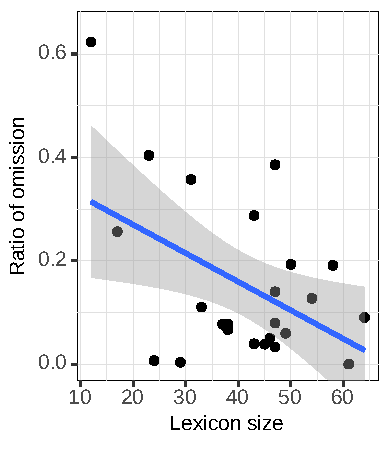
\includegraphics{figures/scr_production_omission_ratio_lexicon}
\end{minipage}
\begin{minipage}{.03\textwidth}
 
\end{minipage}
\begin{minipage}{.48\textwidth}
  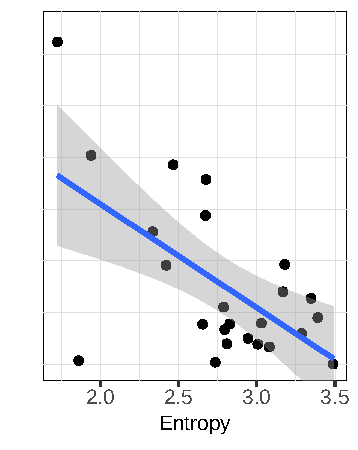
\includegraphics{figures/scr_production_omission_ratio_entropy}
\end{minipage}

 \caption{Ratio of omission as a function of lexicon size and entropy in the script.\label{fig:scripts-ellratio-lexicon}}
\end{figure}

\subsubsection{Variables}
The regression analyses described in what follows investigate effects of the three information-theoretic\is{Information theory} predictors described in the preceding section on the omission of words. \textsc{UnigramSurprisal} models the likelihood of words given extralinguistic context\is{Context, extralinguistic}, \textsc{ContextSurprisal}\is{Shannon information} additionally takes linguistic context\is{Context, linguistic} into account, and \textsc{SurprisalReduction} quantifies how much inserting a word reduces the surprisal\is{Shannon information} of the following one. Additionally, I annotated the position of the word in the utterance (numeric). As I discussed in Section \ref{sec:infotheory-uid}, in the literature there is evidence for optimization of word order\is{Word order} with respect to UID\is{Uniform Information Density}. On average, context\is{Context, linguistic} reduces the information\is{Shannon information} of words, therefore placing more informative\is{Shannon information} words toward the end of the utterance yields a more uniform ID profile\is{Information density}. In Section \ref{sec:scripts-production-results-uniformity}, I show that this prediction is borne out. Table \ref{tab:production-length} provides an overview of the distribution of utterance lengths. All preprocessed utterances had a length between one and five words. As there were only three utterances with a length of five and I analyzed utterance lengths with an ordinal model these three utterances were excluded from further analyses due to data sparseness.

\begin{table}[t]
\begin{tabular}{l p{1cm} p{.9cm} p{.9cm} p{.9cm} p{.9cm}}
\lsptoprule
Length (words) & 1 & 2 & 3 & 4 & 5\\
\midrule
Count & 74 & 680 &1238 & 414& 3\\
\lspbottomrule
\end{tabular}
\caption{Distribution of utterances by length in the production data.\label{tab:production-length}}
\end{table}

\begin{table}[t]
\begin{tabular}{l l l l}
\lsptoprule
Predictors & Pearson's $r^2$ & $t$-value & $p$-value\\
\midrule
Unigram\is{Unigram language model}, context-dependent	& 0.65	& 70.06	& \textless 0.001\\
Unigram\is{Unigram language model}, reduction	& 0.48	& 37.99	& \textless 0.001\\
Context-dependent, reduction	& 0.62	& 54.00	& \textless 0.001\\
\lspbottomrule
\end{tabular}
\caption{Correlations between the information-theoretic predictors.\label{tab:production-correlations}}
\end{table}

\subsubsection{UID effects on omissions in fragments}
\label{sec:scripts-production-results-surprisal}

The data were analyzed with logistic mixed effects regressions predicting the outcome of the binary DV \textsc{Omission} of a word in the enriched data set from the information-theoretic\is{Information theory} measures described above. The analyses were conducted with the \texttt{lme4} package \citep{bates.etal2015} in \texttt{R} and followed the procedure described in Section \ref{sec:intro-stats}: Starting with a full model containing all fixed effects and their two-way interactions as well as a maximal random effects structure, predictors that did not significantly improve model fit (as evidenced by likelihood ratio tests) were successively removed from the model. In principle, it would be desirable to include all three predictors in a single model, but as Table \ref{tab:production-correlations} shows, they are highly correlated and regression analyses require predictors to be independent. Furthermore, effects of \textsc{SurprisalReduc\-tion} cannot be investigated for utterance-final words, which lack a following word whose surprisal\is{Shannon information} they could reduce. Therefore, I conducted three separate regression analyses. The first two analyses investigated whether \textsc{UnigramSurpri\-sal\is{Shannon information}} and \textsc{ContextSurprisal\is{Shannon information}} predict omissions. This would provide evidence for a tendency to avoid troughs in the ID profile\is{Information density}. In the third analysis I tested for an effect of \textsc{Unigram\is{Unigram language model}Surprisal\is{Shannon information}} and \textsc{Surprisal\is{Shannon information}Reduction} simultaneously, which could provide evidence for the avoidance of both peaks and troughs. This analysis was conducted on a subset of the data which excluded the utterance-final words, for which \textsc{Surprisal\is{Shannon information}Reduction} cannot be estimated.

\subsubsubsection{Avoid troughs: Effects of surprisal on omissions}
The density plots in Figures \ref{fig:production_density-unigram}\is{Unigram language model} and \ref{fig:production_density-context}  show the distribution of omissions across the range of \textsc{UnigramSurprisal}\is{Shannon information} and \textsc{ContextSurprisal}\is{Shannon information}. For both measures, the density plots suggest that on average the surprisal\is{Shannon information} of words which have originally been omitted is lower than that of realized words. The effect seems to be more pronounced for \textsc{UnigramSurprisal}\is{Shannon information}. 

\begin{table}[t]
\begin{tabular}{l l l l l l}
\lsptoprule
Predictor & Estimate & SE & $\chi^2$ &  $p$-value &  \\   
\midrule
\textsc{UnigramSurprisal} & -0.337 & 0.117 & 7.39 & \textless 0.01 & **\\
\lspbottomrule
\end{tabular}
\caption{Fixed effects in the final GLMM investigating the effect of \textsc{UnigramSurprisal} on \textsc{Omission}.\label{tab:production-unigram-estimates}}
\end{table}

\begin{table}[t]
\begin{tabular}{l l l l l l}
\lsptoprule
Predictor & Estimate & SE & $\chi^2$ &  $p$-value &  \\   
\midrule
\textsc{ContextSurprisal}\is{Shannon information} & -0.28 &  0.126 &  4.86 & \textless 0.05 & *\\   
\lspbottomrule
\end{tabular}
\caption{Fixed effects in the final GLMM investigating the effect of \textsc{ContextSurprisal} on \textsc{Omission}.\label{tab:production-context-estimates}}
\end{table}

The full model for unigram surprisal\is{Shannon information} contained only a main effect of \textsc{UnigramSurprisal} as well as by-subject and by-item (script) random intercepts and slopes for \textsc{UnigramSurprisal}. The by-subject effects account for individual preferences with respect to omission and the by-item effects for potential differences between scripts\is{Script knowledge}. The \textsc{UnigramSurprisal} main effect was significant \glmer{7.39}{0.01}: The lower the unigram surprisal\is{Shannon information} of a word is, the more likely it is to be omitted (see Table \ref{tab:production-unigram-estimates}). The full model for context-dependent surprisal\is{Shannon information} was identical to the one for unigram surprisal\is{Shannon information} except for the missing by-subject random slope for \textsc{ContextSurprisal}, because the model did not converge otherwise. The effect of \textsc{ContextSurprisal} was significant \glmer{4.86}{0.05} in the final model (see Table \ref{tab:production-context-estimates}).

\begin{figure}[t]
  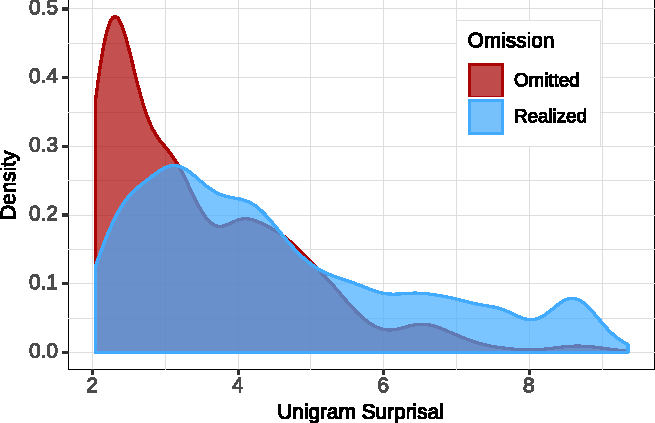
\includegraphics{figures/scr_production_density_unigram}
   \caption{The density plot shows how the omitted and realized words are distributed across the unigram surprisal scale.\label{fig:production_density-unigram}}
\end{figure}

\begin{figure}[t]
  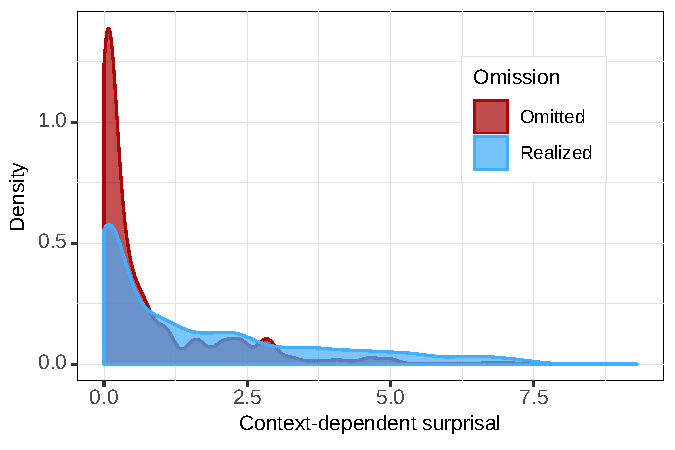
\includegraphics{figures/scr_production_density_context}
     \caption{The density plot shows how the omitted and realized words are distributed across the context-dependent surprisal scale.\label{fig:production_density-context}}
\end{figure}

Taken together, both unigram\is{Unigram language model} and context dependent surprisal\is{Shannon information} predict omissions: Words that are more predictable are more likely to be omitted. This is in line with the prediction of UID\is{Uniform Information Density} that omitting predictable words in order to avoid troughs in the density profile. A somewhat unexpected finding is that \textsc{UnigramSurprisal} seems to be a better predictor of omission than \textsc{ContextSurprisal}. In principle the opposite would be expected, because \textsc{ContextSurprisal} takes more sources of predictability\is{Context, linguistic} into account and should therefore be a more precise measure of predictability. In part, the stronger effect of \textsc{UnigramSurprisal} is probably an artifact of the data set. As the density plot in Figure \ref{fig:production_density-context} shows, the overall distribution of \textsc{ContextSurprisal} is more heavily skewed due to many words having a \textsc{ContextSurprisal} of 0. This results from the relatively small number of complete structures in my data: Sometimes one or two words suffice to completely disambiguate between the structures, so that all following words are fully redundant. An actual speaker however might have a larger set of possible utterances in mind, so that they are not as completely redundant as my model suggests. Therefore, I expect that \textsc{ContextSurprisal} would be a better predictor of \textsc{Omission} if the same procedure is applied to a larger and more diverse data set.

\subsubsubsection{Avoid peaks: Effect of surprisal reduction on omission}

In order to investigate the prediction of UID\is{Uniform Information Density} that redundancy is inserted before unpredictable words in order to smooth peaks, I conducted a third analysis that additionally considers an effect of \textsc{Surprisal\is{Shannon information}Reduction}. This analysis was conducted on a subset of the data that excluded all utterance-final words, for which \textsc{Surprisal\is{Shannon information}Reduction} cannot be estimated, and all words preceding an ellipsis. The latter were excluded because it would be unreasonable to assume that the preceding word reduced the surprisal\is{Shannon information} of an expression that had been omitted in the actual data. The subset used for this analysis contained a total of 3784 words, that is 55.52\% of the total data. The full model contained main effects of \textsc{Surprisal\is{Shannon information}Reduction} and \textsc{Unigram\is{Unigram language model}Surprisal\is{Shannon information}}, the interaction between both IVs and random intercepts for subjects and items. I chose \textsc{Unigram\is{Unigram language model}Surprisal\is{Shannon information}} rather than \textsc{ContextSurprisal\is{Shannon information}} for two reasons: First, it turned out to be a better predictor of omission than \textsc{ContextSurprisal\is{Shannon information}}, and second, as Table \ref{tab:production-correlations} shows, its correlation with \textsc{Surprisal\is{Shannon information}Reduction} is weaker than for \textsc{ContextSurprisal\is{Shannon information}} ($Pearson's\;r^2 = 0.48$ vs. $Pearson's\;r^2 = 0.62$). Table \ref{tab:production-peaks-troughs-estimates} summarizes the final model. The significant main effect of \textsc{UnigramSurprisal} \glmer{10.39}{0.01} replicates the finding of the previous analyses that predictable words are more likely to be omitted. The significant main effect of \textsc{SurprisalReduction} \glmer{27.03}{\highsig} shows that words that reduce the surprisal\is{Shannon information} of the following word more strongly are more likely to be inserted. The interaction between both predictors is not significant \glmernonsig{0.01}{0.9}. Taken together, this shows that optional omissions in fragments are driven by the tendency to avoid both troughs and peaks in the ID profile\is{Information density}, just like UID\is{Uniform Information Density} predicts.

\begin{table}[t]
\begin{tabular}{l l l l l l}
\lsptoprule
Predictor & Estimate & SE & $\chi^2$ &  $p$-value &  \\   
\midrule
\textsc{UnigramSurprisal}   &	-0.151 & 0.046 & 10.39 & \textless 0.01 & **\\
\textsc{Surprisal\is{Shannon information}Reduction} &	-0.349 & 0.07  & 27.03 & \textless \highsig & *** \\
\lspbottomrule
\end{tabular}
\caption{Fixed effects in the final GLMM investigating effects of both \textsc{UnigramSurprisal} and \textsc{SurprisalReduction}.\label{tab:production-peaks-troughs-estimates}}
\end{table}

\subsubsection{UID effects on word order}
\label{sec:scripts-production-results-uniformity}
\is{Word order|(}The production data\is{Production task} also might provide some insights into UID\is{Uniform Information Density} effects on word order\is{Word order}. UID\is{Uniform Information Density} predicts that expressions that are relatively unpredictable in the absence of linguistic context\is{Context, linguistic} tend toward being placed at the end of the utterance, because previous linguistic material reduces their surprisal\is{Shannon information}. There are two ways of testing this prediction empirically at my data set. First, following the line of reasoning taken by \citet{genzel.charniak2002}, if context reduces the surprisal\is{Shannon information} of expressions, words that are more informative\is{Shannon information} in the absence of context should be placed at the end of the utterance because this reduces their information\is{Shannon information} as compared to an initial position. Placing uninformative\is{Shannon information} words at the end of the utterance would reduce their surprisal\is{Shannon information} further and hence increase the risk of a trough in the ID profile\is{Information density}. Therefore, if UID\is{Uniform Information Density} is correct, words with a higher unigram\is{Unigram language model} surprisal\is{Shannon information} that are hence informative\is{Shannon information} in the absence of linguistic context\is{Context, linguistic}, should tend toward appearing at the end of the utterance. Second, the effect of information\is{Shannon information} reduction by preceding linguistic context\is{Context, linguistic} should be reflected in my context-dependent surprisal\is{Shannon information} measure. Therefore, words with a lower context-dependent surprisal\is{Shannon information} are predicted to appear later in the utterance.

\begin{table}[t]
\begin{tabular}{l l l l l l}
\lsptoprule
Predictor & Estimate & SE & $\chi^2$ &  $p$-value &  \\   
\midrule
\textsc{UnigramSurprisal} & \phantom{-}0.475  &  0.057 &  35.47 & \textless \highsig & ***\\
\textsc{ContextSurprisal}\is{Shannon information}  &  -0.585  &  0.054 & 41.78 & \textless \highsig & *** \\
\lspbottomrule
\end{tabular}
\caption{Fixed effects in the final GLMM predicting \textsc{Position} from the surprisal estimates.\label{tab:production-position-estimates}}
\end{table}

These hypotheses were investigated with CLMMs predicting the outcome of an ordinal DV \textsc{Position} with four ordered levels from \textsc{UnigramSur\-prisal} and \textsc{ContextSurprisal}\is{Shannon information}. The analysis was conducted on the complete data set without distinguishing between originally omitted and realized words, because, if fragments are derived from regular sentences, as my experiments in the first part of this book suggest, word order\is{Word order} and omission are in principle independent from each other. Following the procedure applied in previous experiments, I started with a full model that contained main effects for both IVs, their interaction and a full random effects structure. Table \ref{tab:production-position-estimates} summarizes the final model. The position of a word in the utterance is significantly determined by both IVs. Words with a higher \textsc{UnigramSurprisal} tend to appear later \clmmLR{35.47}{\highsig}, whereas words with a higher \textsc{ContextSurprisal}\is{Shannon information} tend to appear earlier \clmmLR{41.78}{\highsig}. Both observations are in line with UID\is{Uniform Information Density}.\is{Word order|)}

\subsubsection{Event likelihood vs. message likelihood}
\label{sec:scripts-production-results-check}
Finally, the production data\is{Production task} can also be used to test the assumption underlying the rating study\is{Acceptability rating task} that utterances referring to predictable events are more likely than those referring to unpredictable ones. If this was not the case, the results of the rating study\is{Acceptability rating task} could not be interpreted as evidence for information-theoretic\is{Information theory} well-formedness perceptions.

I addressed this question by counting how often utterances referring to the messages used in either of the predictability conditions in the rating study\is{Acceptability rating task} were produced in the production study\is{Production task}. There was a large degree of variation between scripts\is{Script knowledge}. For instance, the predictable message was produced in 96.56\% of the trials in the train script, but there were three scripts where it was never produced. Averaging over the production ratios for all scripts shows that the message tested in the predictable condition was still more often produced than that in the unpredictable condition (19.1\% vs. 0.4\% of responses). Note that the estimate for the predictable condition is rather conservative: In three scripts where the speaker buys or orders something, only those messages that refers to the item (s)he orders in the sentential condition in the rating study\is{Acceptability rating task} were counted. Taken together, this clearly confirms the reasoning underlying the rating study\is{Acceptability rating task} that predictable messages are more likely to be talked about.

\subsection{Discussion}

Experiment \ref{exp:scripts-production} provides evidence for the hypothesis that omissions in fragments are driven by a tendency to avoid peaks and troughs in the ID profile\is{Information density}. The main effects of \textsc{UnigramSurprisal} and \textsc{ContextSurprisal}\is{Shannon information} in the statistical analyses show that words that are predictable given extralinguistic\is{Context, extralinguistic} and linguistic context\is{Context, linguistic} are significantly more likely to be omitted. This reflects the tendency to avoid troughs in the ID profile\is{Information density}, which are caused by uninformative\is{Shannon information} words. The main effect of \textsc{SurprisalReduction} indicates that words that reduce the surprisal\is{Shannon information} of the next one are more likely to be realized. This evidences a strategy of reducing peaks in the ID profile\is{Information density} by inserting additional redundancy into the utterance.

Taken together, these findings indicate that UID\is{Uniform Information Density} constrains omissions in fragments. The acceptability rating\is{Acceptability rating task} data from experiment \ref{exp:scripts-rating} are also compatible with a source coding\is{Source coding} account or a general tendency to omit given or redundant material, but none of these accounts predicts the effects of the \textit{following} word's surprisal\is{Shannon information} that experiment \ref{exp:scripts-production} reveals. UID\is{Uniform Information Density} provides a natural explanation for this observation and also accounts for the finding that predictable words themselves are more often omitted.

The observation that predictable words are more likely to be omitted also implies that the choice between a fragment and a full sentence is constrained by UID\is{Uniform Information Density}. Since the experiments show that extralinguistic context\is{Context, extralinguistic} determines the predictability of individual words, the likelihood of a trough that is smoothed by the omission of predictable words is higher in predictive contexts. If the omitted word is required in a full sentence, its omission results in a fragment. This extends previous evidence for UID\is{Uniform Information Density}, where such effects were reported only for highly specific omissions of single closed-class function words to the much more diverse and semantically relevant omissions of content words in fragments. 

Experiment \ref{exp:scripts-production} investigated only omissions of words that cannot be omitted in complete sentence, like verbs and their arguments, whose omission can result in fragments. Aspects of meaning that are conveyed by e.g. temporal or locative adjuncts\is{Adjunct}, which can be implicit in full sentences, might be subject to UID\is{Uniform Information Density} too, however. Just like experiment \ref{exp:scripts-production} showed for words that can be omitted in fragments, adjuncts\is{Adjunct} might also tend to be explicit when they convey less predictable information\is{Shannon information}. Investigating omissions in adjuncts\is{Adjunct} is more complicated, because they are probably more difficult to reconstruct when they are omitted, because a potentially infinite number of adjuncts\is{Adjunct} can be inserted into an utterance. Therefore it is unclear which ones should be reconstructed and which ones should not. In the case of arguments, this reconstruction was more straightforward, because the absence of a syntactically required expression indicates that it must be reconstructed. However, in principle there is no reason to assume that the omission of adjuncts\is{Adjunct} would not be driven by UID\is{Uniform Information Density} as well.

Experiment \ref{exp:scripts-production} also provides evidence for UID\is{Uniform Information Density} effects on word order\is{Word order}. If only unigram\is{Unigram language model} surprisal\is{Shannon information}, which is independent from linguistic context\is{Context, linguistic}, is considered, unpredictable words tend toward appearing late in the utterance, just like \citet{genzel.charniak2002} showed for sentences within a text. This is expected under the assumption that the more linguistic context\is{Context, linguistic} a word has, the more predictable it becomes \citep{genzel.charniak2002, levy2008}. This assumption is in turn confirmed by the inverse effect of my context-dependent surprisal\is{Shannon information} measure which shows that the words at the end of the utterance have a lower context-dependent surprisal\is{Shannon information}. Taken together, the utterances in my data set are constrained by UID\is{Uniform Information Density} in two ways: First, UID\is{Uniform Information Density} constrains the omission of individual words, and second, otherwise unpredictable words are placed toward the end of the utterance, because its surprisal\is{Shannon information} is reduced by preceding material.

\section{The usage of fragments: Discussion}
\label{sec:scripts-discussion}

\subsection{Evidence for UID effects on omissions in fragments}
In this chapter I presented two experiments that investigated the predictions of UID\is{Uniform Information Density} the usage of fragments: (i) that predictable messages are preferably reduced, (ii) that predictable words are more likely to be omitted, and (iii) that words that reduce the surprisal\is{Shannon information} of the next word are more likely to be realized. UID\is{Uniform Information Density} shares the first prediction with source coding\is{Source coding}, but the other two are specific to UID\is{Uniform Information Density}.

Experiment \ref{exp:scripts-rating} supports the first of these predictions by showing that the reduction of predictable utterances is perceived as more well-formed than that of unpredictable ones. Somewhat surprisingly, sentences were on average preferred over fragments in both predictability conditions. This might be due to politeness considerations and the fact that some of the tested fragments are relatively improbable, as evidenced by the production data\is{Production task} collected in experiment \ref{exp:scripts-production}. Nevertheless, the experiment provides first evidence for the hypothesis that the preference for using fragments depends on the predictability of utterances. The design did not allow for the investigation of UID\is{Uniform Information Density} effects on the omission of individual words, therefore the rating study\is{Acceptability rating task} does not ultimately show whether the densification of utterances that encode likely messages is caused by the tendency to avoid peaks and troughs in the ID profile\is{Information density}, as UID\is{Uniform Information Density} predicts.

Experiment \ref{exp:scripts-production} provides evidence for the more fine-grained predictions of UID\is{Uniform Information Density} that speakers avoid peaks and troughs: Words that are themselves predictable are more likely to be omitted and words that reduce the surprisal\is{Shannon information} of following words are more likely to be inserted. The data set based on which these results were obtained was preprocessed to account for grammatical constraints on fragments. Since an optimization with respect to UID\is{Uniform Information Density} has been argued to occur only within the bounds defined by grammar \citep[25]{jaeger2010}, preprocessing ensured that each of the primitive expressions in the data set was equivalent to a constituent whose omission does not structurally depend on surrounding material. For instance, as experiment \ref{exp:pstranding-german} showed that prepositions cannot be freely omitted\is{Preposition omission} in German\is{German}, I merged the noun phrase\is{Noun phrase} and the preposition within a PP\is{Preposition phrase} to a single primitive unit. Experiment \ref{exp:scripts-production} provides clear evidence for UID\is{Uniform Information Density} effects on individual omissions in fragments. This conclusion implies that the choice between producing a fragment and producing a full sentence in a specific situation is also constrained by UID\is{Uniform Information Density}: In unpredictive contexts\is{Context, extralinguistic}, the probability of troughs in the ID profile\is{Information density}, which trigger omissions, is lower than in predictive ones. If no words that are obligatory in full sentences are omitted for this reason, the speaker will prefer to utter a full sentence rather than any of the grammatically possible fragments. This extends previous evidence for UID\is{Uniform Information Density}, where such effects were reported only for highly specific omissions of closed-class function words to the much more diverse omissions of content words in fragments.

Experiment \ref{exp:scripts-production} furthermore provides evidence for UID\is{Uniform Information Density} effects on word order\is{Word order}: Words with a higher unigram\is{Unigram language model} surprisal\is{Shannon information}, which are less predictable in the absence of context, tend to appear late in the utterance. The UID\is{Uniform Information Density} explanation for this observation is that linguistic context\is{Context, linguistic} reduces the surprisal\is{Shannon information} of words that are otherwise unpredictable. Therefore, as \citet{fenk-oczlon1983} argues, placing predictable words before uninformative\is{Shannon information} ones yields a more uniform ID profile\is{Information density}. The assumption that linguistic context\is{Context, linguistic} increases the predictability of words on average is supported by the inverse effect of context-depen\-dent surprisal\is{Shannon information}, where predictable words tend to appear \textit{late} in the utterance. Experiment \ref{exp:scripts-production} thus also provides empirical evidence for a (reasonable) assumption that has only been stipulated in previous work \citep{fenk-oczlon1983, fenk-oczlon1989, genzel.charniak2002}.

\subsection{UID vs. availability-based production}

Following \citet{hale2001}, I assume that the relationship between the likelihood of a word and its omission is determined by processing effort\is{Processing effort}. Speakers perform audience design\is{Audience design} by adapting their message to  the expected cognitive resources of the hearer, and omissions occur whenever they are beneficial to that goal. However, as I sketched in Section \ref{sec:infotheory-uid-competing-abp}, predictability effects have also been explained with the effort required to retrieve a word from memory alone. \is{Availability-based production|(}Availability-based production\is{Availability-based production} predicts that omissions occur more often if the word following the omitted one is predictable and hence easy to retrieve, as \citet{ferreira.dell2000} show for complementizer omission\is{Complementizer omission} in English\is{English}. The same effect is predicted by UID\is{Uniform Information Density}, but for a different reason: Realizing words that precede unpredictable words can reduce the surprisal\is{Shannon information} of the latter and hence smooth peaks in the ID profile\is{Information density}. The observation that words are more likely to be inserted before unpredictable words can therefore be also interpreted as an effect of availability-based production. As \citet{jaeger.buz2017} note, availability-based production and UID\is{Uniform Information Density} are not mutually exclusive and there might be independent effects of both theories, but in case both theories predict the same effect it cannot be attributed unambiguously to either of the theories.

Effects of availability-based production\is{Availability-based production} however are particularly expected in oral communication, because according to \citet{ferreira.dell2000} the motivation for inserting optional words is to avoid disfluencies which would result from the time required to retrieve unpredictable lemmas from memory. This is the case in studies on spoken corpora\is{Corpus} \citep{levy.jaeger2007, frank.jaeger2008, jaeger2010} or spoken production experiments \citep{kurumada.jaeger2015, norcliffe.jaeger2016}, but it does not concern my production study\is{Production task} (experiment \ref{exp:scripts-production}) in the same way: Even though I asked subjects to provide utterances that seem natural in a situation of oral communication, they provided written responses, so there is no risk of disfluencies. Therefore, even though some of the evidence for UID\is{Uniform Information Density} might be explained by production alone, this explanation is less convincing in case of the effects that I found in my production study\is{Production task}.

Furthermore, availability-based production\is{Availability-based production} can only explain why the omission of a target word can be predicted from the surprisal\is{Shannon information} of the following word(s), but not why it depends on the target word's own surprisal\is{Shannon information}. Most of the previous studies on UID\is{Uniform Information Density} and my production study\is{Production task} found that the predictability of the target word itself predicts its omission as well. Taken together, the predictions of UID\is{Uniform Information Density} and availability-based production\is{Availability-based production} partially overlap, and specifically in studies on spoken language some of the effects of UID\is{Uniform Information Density} can be explained by availability-based production\is{Availability-based production} as well. However, availability-based production\is{Availability-based production} cannot account for all of the data, and specifically in my experiments the written modality makes it implausible that omissions depend on the likelihood of disfluencies. This does not speak against the idea of availability-based production\is{Availability-based production}, but it provides distinctive evidence for UID\is{Uniform Information Density}.\is{Availability-based production|)}

\subsection{Information theory or information structure?}
\is{Information theory|(}\is{Information structure|(}The information-theoretic\is{Information theory} account that I pursue often coincides with a perspective based on information structure\is{Information structure}, which requires omitted expressions to be e-given\is{E-givenness} \citep{merchant2004}, not part of the focus \citep{reich2007} or backgrounded \citep{ott.struckmeier2016}. Words that are predictable are probably often given in a possibly implicit QuD\is{Question under Discussion}. For instance, in the taxi example that I used to illustrate my approach above, it is reasonable to assume that a QuD\is{Question under Discussion} like \textit{Where should I take you?} licenses ellipsis of everything but the focused word corresponding to the \textit{wh}-phrase in the answer. From an information-structural\is{Information structure} perspective, given material \textit{can} be omitted because it is given, and from an UID\is{Uniform Information Density} perspective it \textit{should} be omitted, since it would probably yield a trough in the ID profile\is{Information density}. A potential testing ground to distinguish between information structure and information theory are expressions that are given, but not predictable, or vice versa. Givenness and predictability might coincide most of the time though, so that distinguishing between these concepts requires a set of constructed materials for which the predictability of a given expression can be manipulated.

The main difference between an information-theoretic\is{Information theory} and an information-structural\is{Information structure} approach to the usage of fragments, however, is that only information theory\is{Information theory} can  explain why an expression actually is (not) omitted. Information-structural concepts like givenness might license ellipsis, but it is clearly not necessary to omit each given expression. For instance, it is appropriate to answer a question with a full sentence even though most of the words contained in the answer are given. In contrast, UID\is{Uniform Information Density} provides an account of why particular words are preferably omitted and of why they might be realized. Information structure does also not explain why the surprisal\is{Shannon information} of the word that follows a target word has an effect of the target word's omission. This does not neglect the role of information structure on omissions though, and it is very likely that information-theoretic\is{Information theory} concepts like givenness are reflected in and should be taken into account by more sophisticated measures of surprisal\is{Shannon information}.\is{Information theory|)}\is{Information structure|)}

\subsection{Script knowledge as models of extralinguistic context}
Since fragments often appear discourse-initial\is{Fragment, discourse-initial}ly, the predictability of words in context is determined to a large extent by extralinguistic context\is{Context, extralinguistic}, which cannot be captured by standard language modeling techniques applied to speech corpora\is{Corpus}. Therefore, the context stories used in experiments \ref{exp:scripts-rating} and \ref{exp:scripts-production} were based on probabilistic event chain\is{Event chain}s extracted from the DeScript corpus\is{Corpus} of script knowledge\is{Script knowledge} \citep{wanzare.etal2016}, which contains crowdsourced descriptions of the stereotypical time-course of script\is{Script knowledge} events.

The rating study\is{Acceptability rating task} shows that utterances referring to predictable events were more acceptable, and that this holds in particular for fragments. I interpreted this as evidence for optimization of the signal with respect to information-theoretic\is{Information theory} principles because I assumed that predictable events would be more likely to be talked about. The production data\is{Production task} collected in experiment \ref{exp:scripts-production} confirms that this corpus\is{Corpus}-based predictability manipulation in experiment \ref{exp:scripts-rating} is overall in line with subjects' expectations about upcoming utterances. The utterances in the predictable condition in the rating study\is{Acceptability rating task} had an average likelihood  of 19.1\%, whereas those in the unpredictable condition were produced only in 0.4\% of the trials in the production task. Note that this is a conservative estimate since for instance in the pizza ordering scenarios, utterances were classified as encoding a different message depending on what the customer orders.

This manipulation did not work equally well for all scripts\is{Script knowledge}. In three scenarios, the presumably predictable message was never produced and some of the unpredictable fragments that were never produced received relatively high ratings. Consequently, there was no significant correlation between message frequency and the acceptability\is{Acceptability rating task} of fragment conditions. As I discuss in Section \ref{sec:fragments-game} below, the optimality of fragments might not be driven by message frequency alone, but also by the utility of the fragment to unambiguously communicate a message.

On average though, utterances referring to predictable events turned out to be more likely in the production study\is{Production task}. This supports the procedure that I used for constructing materials for experiments \ref{exp:scripts-rating} and \ref{exp:scripts-production} and shows that, even though scripts\is{Script knowledge} do not cover \textit{all} aspects of extralinguistic context\is{Context, extralinguistic}, script\is{Script knowledge} corpora\is{Corpus} provide precise estimates of the likelihood of utterances in context and therefore constitute a empirically sound approximation to extralinguistic context\is{Context, extralinguistic}.

\subsection{Surprisal estimation in elliptical data}

The conclusions drawn from experiment \ref{exp:scripts-production} rely on a novel method to estimate surprisal\is{Shannon information} that is robust to a circularity issue caused by ellipses in the training data: If predictable words are omitted more often, their predictability is not proportional to their corpus\is{Corpus} frequency because they are often omitted. This would distort predictability estimates calculated with regular language models. My approach avoids this problem, because it relies on nonelliptical data for estimating surprisal\is{Shannon information}. The method is similar to the approach proposed by \citet{hale2001}, who derives surprisal\is{Shannon information} from the probability mass of the parses\is{Parser, parallel} that are disconfirmed by an input. Like \citeauthor{hale2001}'s method, it is fully incremental, i.e. the information that a word provides to the parser\is{Parser, human} is used as soon as this word is encountered. The method is also psychologically realistic, because only those words that are available to the hearer are included in the context\is{Context, linguistic} used for surprisal\is{Shannon information} estimation. Words that are omitted in context of the target word have no effect on its surprisal\is{Shannon information}.

The significant effect of context-dependent surprisal\is{Shannon information} in the analysis shows that is a suitable approximation to the information\is{Shannon information} of words in context. However, the effect of unigram\is{Unigram language model} surprisal\is{Shannon information} on omission was stronger than that of context-dependent surprisal\is{Shannon information} even though I expected the opposite because context-depen\-dent surprisal\is{Shannon information} takes more sources of predictability into account. This might be due to the relatively small size of my data set, for which sometimes a sequence of two words completely disambiguates between parses. All following words necessarily receive a surprisal\is{Shannon information} of 0. I expect stronger effects of context-dependent surprisal\is{Shannon information} in larger and more diverse data sets. Linguistic context\is{Context, linguistic} might also be more important when syntactic information, like inflectional marking on verbs, is more prominent. Other measures of context-dependent surprisal\is{Shannon information}, such as word likelihoods derived from a PCFG\is{Context-free grammar} \citep{hale2001} are sensitive to hierarchical syntactic information, such as subcategorization preferences, for instance that of a preposition for a DP\is{Determiner phrase} or specific verbs for a complementizer. Such function words had been removed from my data set during preprocessing.

The data set collected in experiment \ref{exp:scripts-production} was elicited with a set of carefully built context stories and required a considerable amount of manual preprocessing, which consisted in the unification of synonyms, annotation of case morphology and prepositions, removal of adverbials\is{Adverbial} and the reconstruction of ellipses. Since the analysis confirmed the validity of this approach, it might be interesting to explore to which extent it can be automatized, e.g. by automatic unification of synonyms, morphosyntactic annotation and reconstruction of ellipsis. In such research, the manually preprocessed data can be used as a gold standard for the evaluation of automatized preprocessing procedures.

\section[Outline of a game-theoretic model of fragment usage]{Outline of a game-theoretic model of fragment usage}

\label{sec:fragments-game}

This section outlines a possible game-theoretic\is{Game theory} account of fragments, which can potentially explain some aspects of the choice between a fragment and a full sentence that UID cannot. Empirically testing such an account and comparing its predictions to UID\is{Uniform Information Density} is intricate and must therefore be left to future research.

\subsection{Limits of UID effects on the form of utterances}

The regression approach that I took in the analysis of experiment \ref{exp:scripts-production} predicts the omission of individual words within a complete sentence from information-theoretic\is{Information theory} variables, such as the surprisal\is{Shannon information} of the target word or how much this word's insertion reduced that of the word following it. However, as I noted in section \ref{sec:infotheory-uid}, UID\is{Uniform Information Density} faces an empirical problem when a single fragment can be derived from a predictable and an unpredictable sentence. For the purpose of illustration, consider the situation where the fragment in \Next[a] is used to communicate the full sentences in \Next[b] or \Next[c] in the taxi scenario discussed above (the probabilities associated with each complete structure are hypothetical).

\ex. \a. To the university.
    \b. Take me to the university. \hfill $p = 0.2$
    \c. Tell me the way to the university.\hfill $p = 0.05$
    \d. [other messages, cumulated] \hfill $p = 0.75$

This issue concerns the usage of the fragment in order to communicate \Last[c]. The ID profile Figure \ref{fig:fragments-uid-unpredictable} suggested that omitting \textit{tell me the way} would result in a peak in the ID profile\is{Information density} that can be avoided by inserting these words, but I already noted there that this is a simplification. Since a hearer who perceives the fragment in \Last[a] does not know whether it has been derived from \Last[b] or \Last[c], processing the fragment must be equally effortful\is{Processing effort} in both cases. Therefore, the fragment will either exceed channel capacity in both cases or in neither of them. %

The problem with encoding the unpredictable \Last[c] with the fragment in \Last[a] therefore is not a peak in the ID profile\is{Information density}, but that a hearer who encounters the fragment in the scenario in \Last has to guess whether the speaker intended to convey \Last[b], \Last[c] or another message. Intuitively, he will go for the more likely \Last[b],% 
% 
\footnote{Only those messages that a fragment can potentially encode will be considered, i.e. those from which the fragment can be derived by ellipsis. For instance, \Last[a] can be derived from \Last[b] and \Last[c], whereas \textit{Take me to the airport} is not a possible source for \Last[a].}\afterfn%
%
because the speaker is more likely to intend to communicate this message than \Last[c]%
%
\footnote{Note that this is also in line with the source coding\is{Source coding}-based prediction that more frequent messages are assigned shorter codes.}\afterfn%
%
and the hearer is consequently more likely to interpret the utterance as intended. UID\is{Uniform Information Density} is by definition unable to take this difference between meanings into account because it models only the encoding procedure, i.e. the choice of the most well-formed utterance to communicate a specific message given the properties of the communication system. Decodingm, the choice of a message given a received signal, is simply not covered by UID\is{Uniform Information Density}.

Before discussing a potential solution to this issue, note that this is a conceptual problem rather than an empirical one. The speaker does neither know with certainty the capacity\is{Channel capacity} of the channel nor the hearer's probability distribution over possible complete structures that determines surprisal\is{Shannon information}. Therefore, all she can do is omit words that are \textit{more likely} to yield a trough and to insert those that are \textit{more likely} to smooth a peak in the ID profile\is{Information density}. From this perspective, she will omit the predictable \textit{take me} in \Last[b] and realize the less predictable \textit{tell me the way} in \Last[c]. The unpredictable \textit{to the university} will be preferably realized in both situations.

\subsection{Game-theoretic pragmatics}
\is{Game theory|(}A framework that might overcome this problem is game-theoretic\is{Game theory} pragmatics. Game-theoretic approaches provide a model of context\is{Context, extralinguistic} which takes into account the knowledge and preferences of rational agents. The model allows for determining which action is the most useful one to pursue for each of the agents. Such models have been recently gaining popularity in pragmatics and been applied to phenomena like implicature \citep{vanrooy2004, benz.vanrooij2007, franke2009, jager2012, goodman.stuhlmuller2013, gotzner.benz2018} and reference \citep{frank.goodman2012, rohde.etal2012, sikos.etal2019}. \is{Iterated Best Response model|(}In what follows I base my expositions on the approach taken by \citet{franke2009}, who develops a game-theoretic\is{Game theory} account of pragmatic reasoning that models implicatures, the \textit{Iterated Best Response} (IBR\is{Iterated Best Response model}) model. He interprets communicative situations as signaling games, which are played by a speaker and a hearer and require a speaker to pick an utterance in order to get a message across.%
%
\footnote{The terminology used in the game-theoretic\is{Game theory} literature differs from the one that I use, which I maintain in order to keep the mapping between terms and concepts throughout this book. In the game-theoretic\is{Game theory} literature, the utterance is called the \textit{message} and what is being communicated (I use the term \emph{message} for this) is labeled the \textit{state}.}\afterfn%
%
Even though Franke investigates a different phenomenon, the problem of mapping utterances and interpretations remains the same, so in principle it can be straightforwardly applied to the interpretation of fragments.

The main ingredients of a signaling game are a set of possible messages, i.e. meanings that the speaker could intend to communicate, a set of possible interpretation actions, that is, meanings that the hearer could assign the utterance and a set of utterances that can be used for this purpose. Only the speaker knows with certainty which message she wants to convey, and she has to choose the utterance that she believes to be the best one to get a message across. The hearer has to figure out which message the speaker intended to communicate. In this setting, both the speaker and the hearer initiate a chain of recursive reasoning about each other which result in the choice of an utterance and the assignment of a meaning (a message) to this utterance. Which utterance is most optimal from the speaker perspective and which meaning the hearer assigns to it depends on a series of parameters: First, the messages often differ in their \textit{prior probability} before any utterance is produced. In the case of the taxi example, it might be more likely that people would ask for a ride than that they would ask for directions. Second, the production of some utterances can be more effortful and hence costly. Third, a single utterance can sometimes encode more than one message, and a single message can be referred to by more than one utterance. Finally, game-theoretic\is{Game theory} models may include varying payoffs that each participant receives depending on her own and the other player's choices. In linguistic applications, where the speaker wants to get a message across and the hearer wants to figure it out correctly, the payoffs for both interlocutors are aligned, since both share the goal of successful communication \citep[21]{franke2009}. In what follows I present a simplified sketch of how \citet[59--61]{franke2009} applies this model to scalar implicature before I illustrate how this reasoning can be extended to fragments.

\subsection{Game-theoretic modeling of scalar implicatures}
For scalar implicatures, \citet{franke2009} focuses on the interpretation of the quantifier \textit{some} as \textit{some but not all}. Despite theoretical and empirical debates on how exactly this interpretation is generated \citep[see e.g.][]{levinson1983, levinson2000, sperber.wilson1986, vankuppevelt1996, breheny.etal2006, huang.snedeker2009, grodner.etal2010}, the general observation is that utterances like \Next[a] are often interpreted as \Next[b], even though semantically \Next[a] is implied by and hence does not rule out \Next[c].

\ex. \a. Some of students completed the assignment.
     \b. Some but not all of the students completed the assignment.
     \c. All of the students completed the assignment.

\citet[59--61]{franke2009} models this situation with a reference game, whose parameters are given in Table \ref{tab:gt-si}. In the game there are only two possible meanings, $m_{\exists\neg\forall}$ and  $m_{\forall}$, two corresponding interpretation actions $a_{\exists\neg\forall}$ and  $a_{\forall}$ and two possible utterances, $u_{some}$ and $u_{all}$. The two utterances correspond to \Last[a,c] respectively. Whereas $u_{some}$ is true in case of both messages, $u_{all}$ is false if $m_{\exists\neg\forall}$ is true. Therefore, $u_{all}$ may be selected only if that the speaker wants to communicate that all students completed the assignment. Each of the messages has a prior probability $Pr(m)$. As I noted above, under the assumption that both agents pursue the goal of successful communication, the payoffs for speaker and hearer are matched: Both receive a payoff of 1 if the interpretation action corresponds to the intended message and no payoff if it does not.
     
\begin{table}[t]
 \begin{tabular}{l c c c c c c}
 \lsptoprule
  & Pr(m) & $a_{\exists\neg\forall}$ & $a_{\forall}$ & $u_{some}$ & $u_{all}$\\
  \midrule
 $m_{\exists\neg\forall}$ & 1 -- p & 1,1 & 0,0 & \ding{51} & -- \\
  $m_{\forall}$ & p & 0,0 & 1,1 & \ding{51} & \ding{51} \\
  \lspbottomrule
 \end{tabular}
 \caption{Tableau for the scalar implicature game, adapted from \citet[21]{franke2009}. The table provides the probability $Pr(m)$ for each message, the speaker and hearer payoffs for each combination of messages and interpretation actions and determines which utterance can be used to communicate each message.\label{tab:gt-si}}
 \end{table}
 
Based on this setting, two chains of iterative reasoning of the agents about each other's behavior are initialized. One of these chains starts with a \textit{literal} speaker and the other one with a literal hearer. Unlike higher order \textit{pragmatic} agents, literal agents take only the general setup of the model into account but do not reason about the other agent's behavior. The literal speaker selects randomly an utterance that is true. In order to communicate $m_{\exists\neg\forall}$, the only available utterance is $u_{some}$, because $u_{all}$ is false in this situation. In contrast, $m_{\forall}$ can be communicated with both utterances, because both are true for this message. This yields the following \textit{strategies}:


\begin{equation}
S_0 = \begin{Bmatrix} t_{\exists\neg\forall} \mapsto m_{some}\\
        t_{\forall} \mapsto m_{some}, m_{all}\\
       \end{Bmatrix}
\end{equation}

The literal hearer calculates the posterior probability of each message to be intended by the speaker given each of the available utterances. The listener does not reason about the speaker's behavior and considers only the prior probability of each message and the truth conditions. In the first sketch of his approach, \citet{franke2009} uses flat priors ($p = 0.5$). Table \ref{tab:gt-si-l0} summarizes the posterior probabilities for the scalar implicature game. If the hearer encounters $u_{all}$, the posterior probability of $\mu(m_{\exists\neg\forall}|u_{all})$ equals 0, because the utterance would be false in case of the message. Therefore, $\mu(m_{\forall}|u_{all}) = 1$, because this is the only message for which $u_{all}$ is true. If the hearer encounters $u_{some}$, both messages could be true, so he will go for the most likely one in order to maximize the likelihood of figuring out the intended meaning. Since both messages are equally likely in case of flat priors, assigning an interpretation to the utterance consists in random guessing.%
%
\footnote{However, if $m_{\exists\neg\forall}$ is more likely than $m_{\forall}$ (if $p > 0.5$), assuming that the more likely message was intended increases the probability of success.}\afterfn%
%
This yields the interpretation strategies in Table \ref{tab:gt-si-l0}: $u_{some}$ will be interpreted either as $m_{\exists\neg\forall}$ or $m_{\forall}$, whereas $u_{all}$ will be always interpreted as $m_{\forall}$:

\begin{table}[t]
\begin{tabular}{c c c}
 \lsptoprule
 $\mu_0(m|u)$ & $m_{\exists\neg\forall}$ & $m_{\forall}$\\
\midrule
$u_{some}$ & ½ & ½ \\
$u_{all}$ & 0 & 1\\
\lspbottomrule
\end{tabular}
\caption{Posterior probabilities for the literal hearer $L_0$.\label{tab:gt-si-l0}}
\end{table}
%
%
\begin{equation}\label{eq:l0}
 L_0 = \begin{Bmatrix} u_{some} \mapsto m_{\exists\neg\forall},m_{\forall}   \\
        u_{all} \mapsto m_{\forall}\\
       \end{Bmatrix}
\end{equation}

The pragmatic speaker takes into account these interpretation strategies of the literal hearer. Since the hearer will unambiguously interpret $u_{all}$ as $m_{\forall}$ but might understand $u_{some}$ as either of the messages, $u_{all}$ has a higher \textit{utility} than $u_{some}$ to communicate $m_{\forall}$. In order to communicate $m_{\exists\neg\forall}$ the utility of $u_{all}$ is 0. Even though a literal hearer might interpret $u_{some}$ as $m_{\forall}$ half of the time, $u_{some}$ is the more promising option for the speaker to get the message across. This results in the following strategies:

\begin{equation}
 S_1 = \begin{Bmatrix} t_{\exists\neg\forall} \mapsto m_{some}\\
        t_{\forall} \mapsto m_{all}\\
       \end{Bmatrix}
\end{equation}

The pragmatic hearer calculates the posterior probability for each message given each utterance, but unlike $L_0$ he takes not only the priors but also the strategies of $S_0$ into account. He calculates the product between the prior probability of a message $m$ and $S_0$ uses a $m$ to encode this message, which is divided by the sum of this term for each message in this situation that $u$ could potentially encode as well \citep[27]{franke2009}:

\begin{equation}
\displaystyle \mu(m|u) = \frac{Pr(m) \times \sigma (u|m)}{\sum_{m'\in M} Pr(m') \times \sigma(u|m')} %)
\end{equation}

This measure increases the higher the prior probability of $m$ is and the more likely $u$ is to be used to encode $m$ as compared to the alternative messages $m'$. In the case of the scalar implicature this yields the posterior probabilities in Table \ref{tab:gt-si-l1}, which, applying the same reasoning as above, result in the interpretation strategies that are in line with the encoding preferences of $S_1$ \ref{eq:gt_l1}:%
%
\footnote{For a more detailed discussion of the formula see \citep[26--27]{franke2009} and for the application to scalar implicatures \citep[60]{franke2009}.}\afterfn%
%

\begin{table}[t]
\begin{tabular}{c c c}
 \lsptoprule
 $\mu_0(m|u)$ & $m_{\exists\neg\forall}$ & $m_{\forall}$\\
\midrule
$u_{some}$ & ⅔ & ⅓ \\
$u_{all}$ & 0 & 1\\
\lspbottomrule
\end{tabular}
\caption{Posterior probabilities for the pragmatic hearer $L_1$.\label{tab:gt-si-l1}}
\end{table}

\begin{equation}
L_1 = \begin{Bmatrix} u_{some} \mapsto m_{\exists\neg\forall} \\
        u_{all} \mapsto m_{\forall}\\
       \end{Bmatrix}\label{eq:gt_l1}
\end{equation}

This model is of course highly simplified because it avoids further alternative expressions and interpretations, such as other quantifiers (\textit{many}, \textit{most}, etc.) and the more explicit, but longer \textit{some but not all}.%
%
\footnote{Effects of a \textit{some but not all} message are discussed by \citet[77, 127]{franke2009}.}\afterfn%
%
Still though, it can model scalar implicatures both on the side of the hearer and on that of the hearer after only one recursive iteration step. The strategies of $L_1$ or $S_1$ can also be the input to higher order reasoning processes.\is{Iterated Best Response model|)}\is{Game theory|)}

\subsection{Application to fragments}
The case of fragments is often more complex than the (simplified) scalar implicature example discussed above. However, the underlying situation is similar, even though the set of messages and utterances is considerably larger: There is a set of possible messages that the speaker might want to communicate to the hearer and a set of utterances that she can use for this purpose. The sets of possible messages and utterances are potentially extremely large (if not infinite, due to recursion in language), but in situations that are constrained by script knowledge\is{Script knowledge} (like in the data from experiment \ref{exp:scripts-production}), the set of actually considered alternative messages and utterances is often relatively limited.  Consider a simplified version of the pasta scenario which I used to illustrate the surprisal calculation methods in Section \ref{sec:scripts-production-surprisal}. In this version of the scenario there are only two messages with differing prior probabilities, which are given in \Next. Again, I use the representations that resulted from preprocessing the production data\is{Production task} collected with experiment \ref{exp:scripts-production}. Each message $m_i$ has is associated a (hypothetical) prior probability $Pr(m_i)$.

\ex. \a. \texttt{pour pasta pot} \hfill $Pr = 0.6$
     \b. \texttt{pour salt pot} \hfill $Pr = 0.4$

Under the assumption that each ``word'' in these utterances can be omitted independently from the surrounding words, the set of possible utterances is:

\begin{equation}
 U = \begin{Bmatrix}
       pour \mathspace pasta \mathspace pot, pour \mathspace salt \mathspace pot,\\
       pour \mathspace pasta, pour \mathspace pot, pour \mathspace salt, pasta \mathspace pot, salt \mathspace pot,\\
       pour, pasta, pot, salt
      \end{Bmatrix}
\end{equation}

Even in this highly simplified scenario with only two messages that differ only in one word, there are 11 possible utterances. The combination with the two messages in \Last yields the tableau in Table \ref{tab:gt-fragments-truth}, based on which the same reasoning steps like in the scalar implicature example can be performed. If more meanings were considered, the complexity of the tableau would increase, but the problem remains identical.

\begin{table}[t]
\begin{tabular}{l l p{.34cm} p{.34cm} p{.21cm} p{.21cm} p{.21cm} p{.21cm} p{.21cm} p{.21cm} p{.21cm} p{.21cm} p{.21cm} p{.21cm} p{.21cm} p{.21cm}}
\lsptoprule
Message & Pr(m) & \rotatebox{90}{$a_{pour \mathspace pasta \mathspace pot}$} & \rotatebox{90}{$a_{pour \mathspace salt \mathspace pot}$} & \rotatebox{90}{\texttt{pour pasta pot}} & \rotatebox{90}{\texttt{pour salt pot}} & \rotatebox{90}{\texttt{pour pasta}} & \rotatebox{90}{\texttt{pour pot}} & \rotatebox{90}{\texttt{pour salt}} & \rotatebox{90}{\texttt{pasta pot}} & \rotatebox{90}{\texttt{salt pot}} & \rotatebox{90}{\texttt{pour}} & \rotatebox{90}{\texttt{pasta}} & \rotatebox{90}{\texttt{pot}} & \rotatebox{90}{\texttt{salt}}\\
\midrule
$m_{pour \mathspace pasta \mathspace pot}$ & 0.6 & 1,1 & 0,0 & \ding{51} & -- & \ding{51} & \ding{51} & -- & \ding{51} & -- & \ding{51} & \ding{51} & \ding{51} & --  \\
$m_{pour \mathspace salt \mathspace pot}$ & 0.4 & 0,0 & 1,1 & -- & \ding{51} & --  & \ding{51} & \ding{51} & --  & \ding{51} & \ding{51} & -- & \ding{51} & \ding{51}\\
\lspbottomrule
\end{tabular}
\caption{Tableau for the simplified pasta scenario game. \label{tab:gt-fragments-truth}}
\end{table}

Applying game-theoretic\is{Game theory} reasoning to the production and interpretation of fragments requires a conceptual and a methodological modification to the approach by \citet{franke2009}. The theoretical modification concerns the relationship between utterances and messages. In the case of \citeauthor{franke2009}'s model, there are only complete utterances, and truth conditions determine whether an utterance is suitable for communicating a message. In the case of fragments however, it is not reasonable to assume that a noun phrase\is{Noun phrase} like \textit{pasta} is \textit{true} in a situation. Instead, the relationship between utterances and messages can be modeled by the suitability of an utterance to communicate a message: An utterance is classified as suitable for communicating a message if it can be derived by an arbitrary number of omissions from the message's full form: \texttt{pour pasta} can be derived from $m_{pour \mathspace pasta \mathspace pot}$ by omitting \texttt{pot}, whereas it cannot be derived from $m_{pour \mathspace salt \mathspace pot}$. Of course, this is a further simplification, because in reality each message can be encoded by a variety of nonelliptical utterances, which differ in the choice of lexical items and word order, among other properties. However, in principle the same reasoning can be applied to this situation: The set of utterances that can encode a message is restricted to those expressions that can be generated by grammatically licensed omissions from the set of full sentences that can encode this message.

The methodological problem concerns ambiguous\is{Ambiguity} fragments. Since speakers use fragments, so it is reasonable to assume that in some situations fragments are more useful encodings than full sentences, so the model must allow for this outcome. However, the model so far predicts that fragments are sometimes as good as sentences, but never better than them: Complete sentences unambiguously identify the message intended by the hearer, so they are always preferred over potentially more vague fragments, just like the unambiguous\is{Ambiguity} $u_{all}$ has the highest utility in the scalar implicature game by \citet{franke2009}. Even though, at least in the example presented here, fragments like e.g. \texttt{salt} or \texttt{pasta} share this property, in this situation they are not preferred over the full sentence. The main advantage of fragments is that they perform the same function as sentences in less time and with a reduced production effort for the speaker. Therefore, it is reasonable to integrate a cost term into the model, which reduces the speaker utility of longer utterances by discounting a percentage of the utility for each word. This models the speaker's preference for producing shorter utterances, which will favor unambiguous\is{Ambiguity} fragments in the case of my example. In large-scale applications the cost term might even favor potentially ambiguous\is{Ambiguity} fragments, if the prior probability of the message as compared to competing messages and the reduction of production cost are large enough to outweigh the remaining ambiguity\is{Ambiguity}.

\subsection{Application to natural language data}
In principle it is possible to apply this model to the data set collected with experiment \ref{exp:scripts-production}. This data set contains an annotation layer of the message underlying each utterance, so that the prior probability of each of message in the scenario can easily be calculated. Based on the preprocessed data set it is also straightforward to determine which complete structures can used to communicate each message and hence to specify (i) the set of possible utterances and (ii) whether each of these utterances can be used to communicate a message. However, the simple example above showed that even when there are only two possible messages there are 11 possible utterances. Consequently, the about 100 utterances produced for each scenario in experiment \ref{exp:scripts-production} do not allow for a fine-grained investigation of the relationship between game-theoretic\is{Game theory} utility and omission. A larger and more homogeneous data set would be required to investigate the predictions of a game-theoretic\is{Game theory} account of fragment usage in detail.

\subsection{Implications and comparison to UID}
Even though I argued in the introduction to this section that UID\is{Uniform Information Density} and game theory\is{Game theory} make partially overlapping predictions on omissions in fragments, they differ with respect to which aspects of communication they model, the mechanism that derives their predictions, and some empirical predictions.

Game theoretic pragmatics\is{Game theory} models both the behavior of the speaker and the hearer, whereas UID\is{Uniform Information Density} focuses on the speaker and accounts only for encoding but not for decoding. The hearer is taken into account indirectly, since the speaker adapts the signal to the cognitive resources\is{Processing effort} she assumes the hearer to possess. The game-theoretic approach explicitly models the actions performed by both agents, as well as their expectations and preferences. By focusing on encoding, UID\is{Uniform Information Density} compares and ranks the usefulness of various utterances to communicate a single message, and the properties and the likelihood of alternative messages are considered only insofar as they contribute to the surprisal\is{Shannon information} of words. This ignores the possibility that an utterance is falsely interpreted as another message than the one intended by the speaker. In contrast, the game-theoretic account predicts a preference for more explicit forms if the intended interpretation is not the most likely one if a fragment was used.

UID\is{Uniform Information Density} and the game-theoretic\is{Game theory} approach also attribute production preferences to different mechanisms. Whereas UID\is{Uniform Information Density} is a psycholinguistic theory based on the efficient distribution of processing effort\is{Processing effort} (in the interpretation that I adopt) or efficient communication in the presence of noise and is relatively indifferent to meaning, a game-theoretic approach does not take into account processing explicitly but focuses on the mapping between utterances and meanings. Even though I showed above that the predictions of UID\is{Uniform Information Density} and game theory are often aligned, the different mechanisms that trigger the choice of an encoding result in partially diverging predictions with respect to the insertion of additional redundancy to avoid troughs: From a game-theoretic\is{Game theory} perspective, a maximally informative fragment is the optimal encoding, whereas from the UID\is{Uniform Information Density} perspective it can be beneficial to insert redundant material in such an utterance in order to reduce peaks in the ID profile\is{Information density} even though these insertions do not increase the utility of the utterance from a game-theoretic\is{Game theory} perspective. The evidence from previous research and my experiments that speakers avoid peaks in the ID profile\is{Information density} suggests that a game-theoretic\is{Game theory} account alone cannot account for the complete empirical picture and a processing account like UID\is{Uniform Information Density} is still needed.

Since UID\is{Uniform Information Density} and the game-theoretic\is{Game theory} approach operate on different levels of analysis and model different aspects of language production and comprehension, they are not mutually exclusive. Furthermore, each of the approaches can account for empirical observations that the other one cannot: UID\is{Uniform Information Density} predicts that speakers insert additional redundancy before unpredictable words, and the game-theoretic\is{Game theory} account explains why peaks in the ID profile\is{Information density} are not smoothed by omitting unlikely words. Therefore, in future research both approaches might be integrated in a more comprehensive model of the choice between alternative ways of encoding a message. For instance, the well-formedness with respect to UID\is{Uniform Information Density} might be included in the game-theoretic\is{Game theory} model as a cost term that penalizes inefficient signals. Since the speaker has an interest in getting her message across, she will try to prevent communication failure resulting from violations of UID\is{Uniform Information Density}. Future research might spell out such an account and test its empirical predictions.
